\chapter{分布式对象存储系统管控平台概要设计}

% 本章主要阐述了系统架构、系统各模块具体架构和数据库概要设计等方面的内容,通过借助系统结构图和活动图来描述各功能实现的基本原理,为第五章的详细设计奠定了基础。

本章对系统的整体架构、系统各功能模块的详细架构以及数据库概要设计等方面的内容作了细致的阐述,通过系统结构图与活动图来说明各功能实现的基本原理,为第五章系统的详细设计打下了基础。


\section{系统架构设计}

根据微服务的拆分原则,可将系统的功能拆分为四大模块,分别是存储管理模块、权限控制模块、认证中心模块和API网关模块。系统整体的逻辑架构如图\ref{fig:系统逻辑架构图}所示。
\begin{figure}[h]
    \centering
    \includegraphics[width=0.8\textwidth]{my_figures/chapter4/系统逻辑架构图.png}
    \caption{系统逻辑架构图}
    \label{fig:系统逻辑架构图}
%     \note{注:图注的内容不宜放到图题中。}
\end{figure}

根据系统逻辑架构图可知,存储管理、权限控制和认证中心是通过API网关与前端进行交互的三个微服务,API网关是系统的大门,同时也是唯一暴露给外部的端口。当请求访问网关微服
务端口时,首先要经过认证中心进行身份校验,确保用户信息的准确无误。权限控制模块主要负责管理用户的账户、角色和权限等信息。存储管理模块是整个管控系统的核心服务,同时
也与MySQL数据库和对象存储系统服务器相连接。MySQL数据库中存储管控平台上使用者的账户、角色和权限等相关信息,而对象存储服务器则是用户上传或下载文件的位置,是整个系统
最为关键的部分。

\section{系统功能模块架构}

\begin{figure}[h]
    \centering
    \includegraphics[width=0.8\textwidth]{my_figures/chapter4/系统功能模块图.png}
    \caption{系统功能模块图}
    \label{fig:系统功能模块图}
%     \note{注:图注的内容不宜放到图题中。}
\end{figure}

基于软件工程的高内聚、低耦合的思想,将分布式对象存储系统管控平台划分为五个模块:注册认证、权限控制、策略控制、文件存取和系统监控。每个模块下又包含多个功能子模块,
例如,注册认证模块包括用户注册子模块、用户登录子模块和身份认证子模块;权限控制模块包括权限管理子模块、角色管理子模块和网关鉴权子模块;策略控制模块包括用户管理子
模块、策略管理子模块和策略分配子模块;文件存取模块包括桶管理子模块、文件上传子模块和文件下载子模块;系统监控模块包括状态监测子模块、事件追踪子模块和告警通知子模
块。系统的功能模块图如图 \ref{fig:系统功能模块图}所示。

可以看出,系统的功能模块图与系统用例表中对模块的划分并不完全一致。原因在于系统用例表是根据用户需求表进行抽象得出的系统用例,而功能模块图是从系统实现的角度出发,以
软件工程中的项目开发思想划分系统功能。以策略控制模块为例,系统要进入此模块,首先需要经过注册认证模块。而对于策略控制过程来说,为了实现管理系统的可扩展性,在管理系
统底层添加了大量子流程;这些子流程中依次使用了网关鉴权功能、注册认证功能以及策略控制模块这三种功能。用户对这些子过程的发生是不可感知的,这些访问过程对于用户来说是
透明的。通常,在系统用例表中的每个用例的实现都需要一个或多个模块的协同配合才能完成。

\section{系统各功能模块设计}

\subsection{注册认证模块}



\begin{figure}[h]
    \centering
    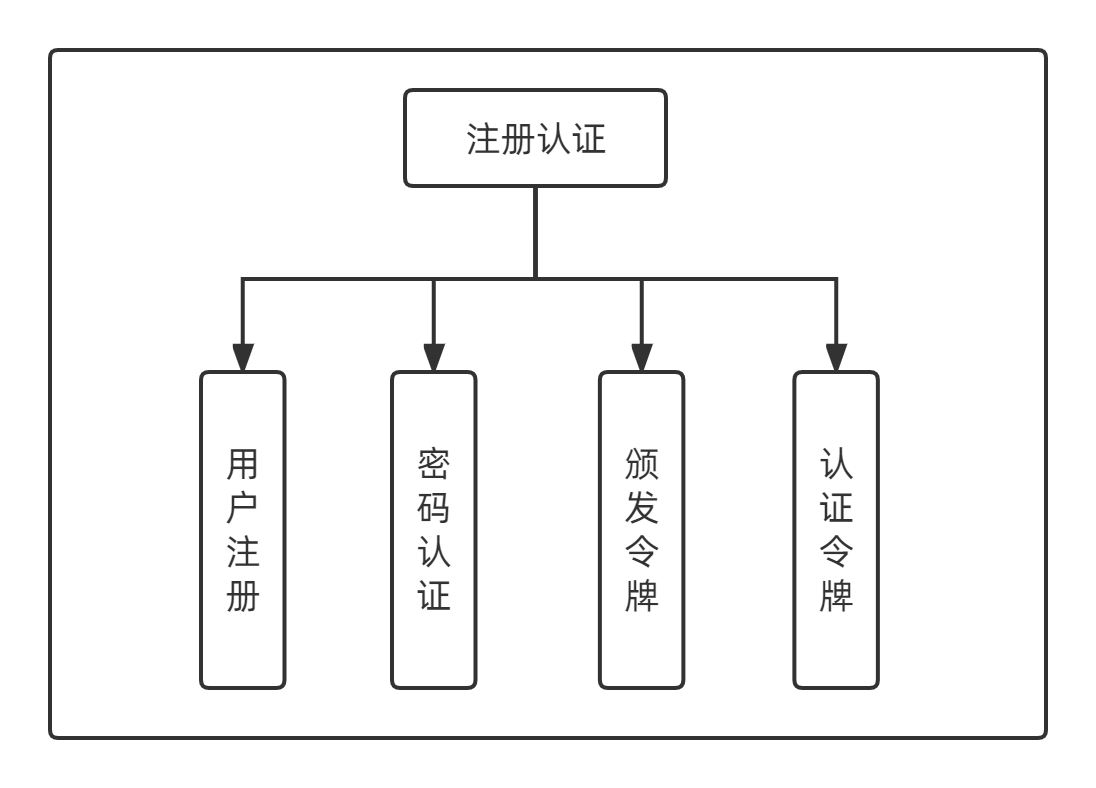
\includegraphics[width=0.5\textwidth]{my_figures/chapter4/注册认证模块功能结构图.png}
    \caption{注册认证模块功能结构图}
    \label{fig:注册认证模块功能结构图}
%     \note{注:图注的内容不宜放到图题中。}
\end{figure}

注册认证模块主要包含用户注册、用户登录、身份认证三个子功能模块。注册认证模块的功能结构图如图\ref{fig:注册认证模块功能结构图}所示。



(1)用户注册

本系统的登录用户共有三种,分别是系统管理员、企业管理员和普通用户。其中,系统管理员不需要注册,因为在项目部署初期,它会由开发人员创建。相反,企业管理员和普通用户需要进行用户注册。企业管理员由于其特殊身份,在注册过程中会有一些特殊限制。
\begin{figure}[h]
    \centering
    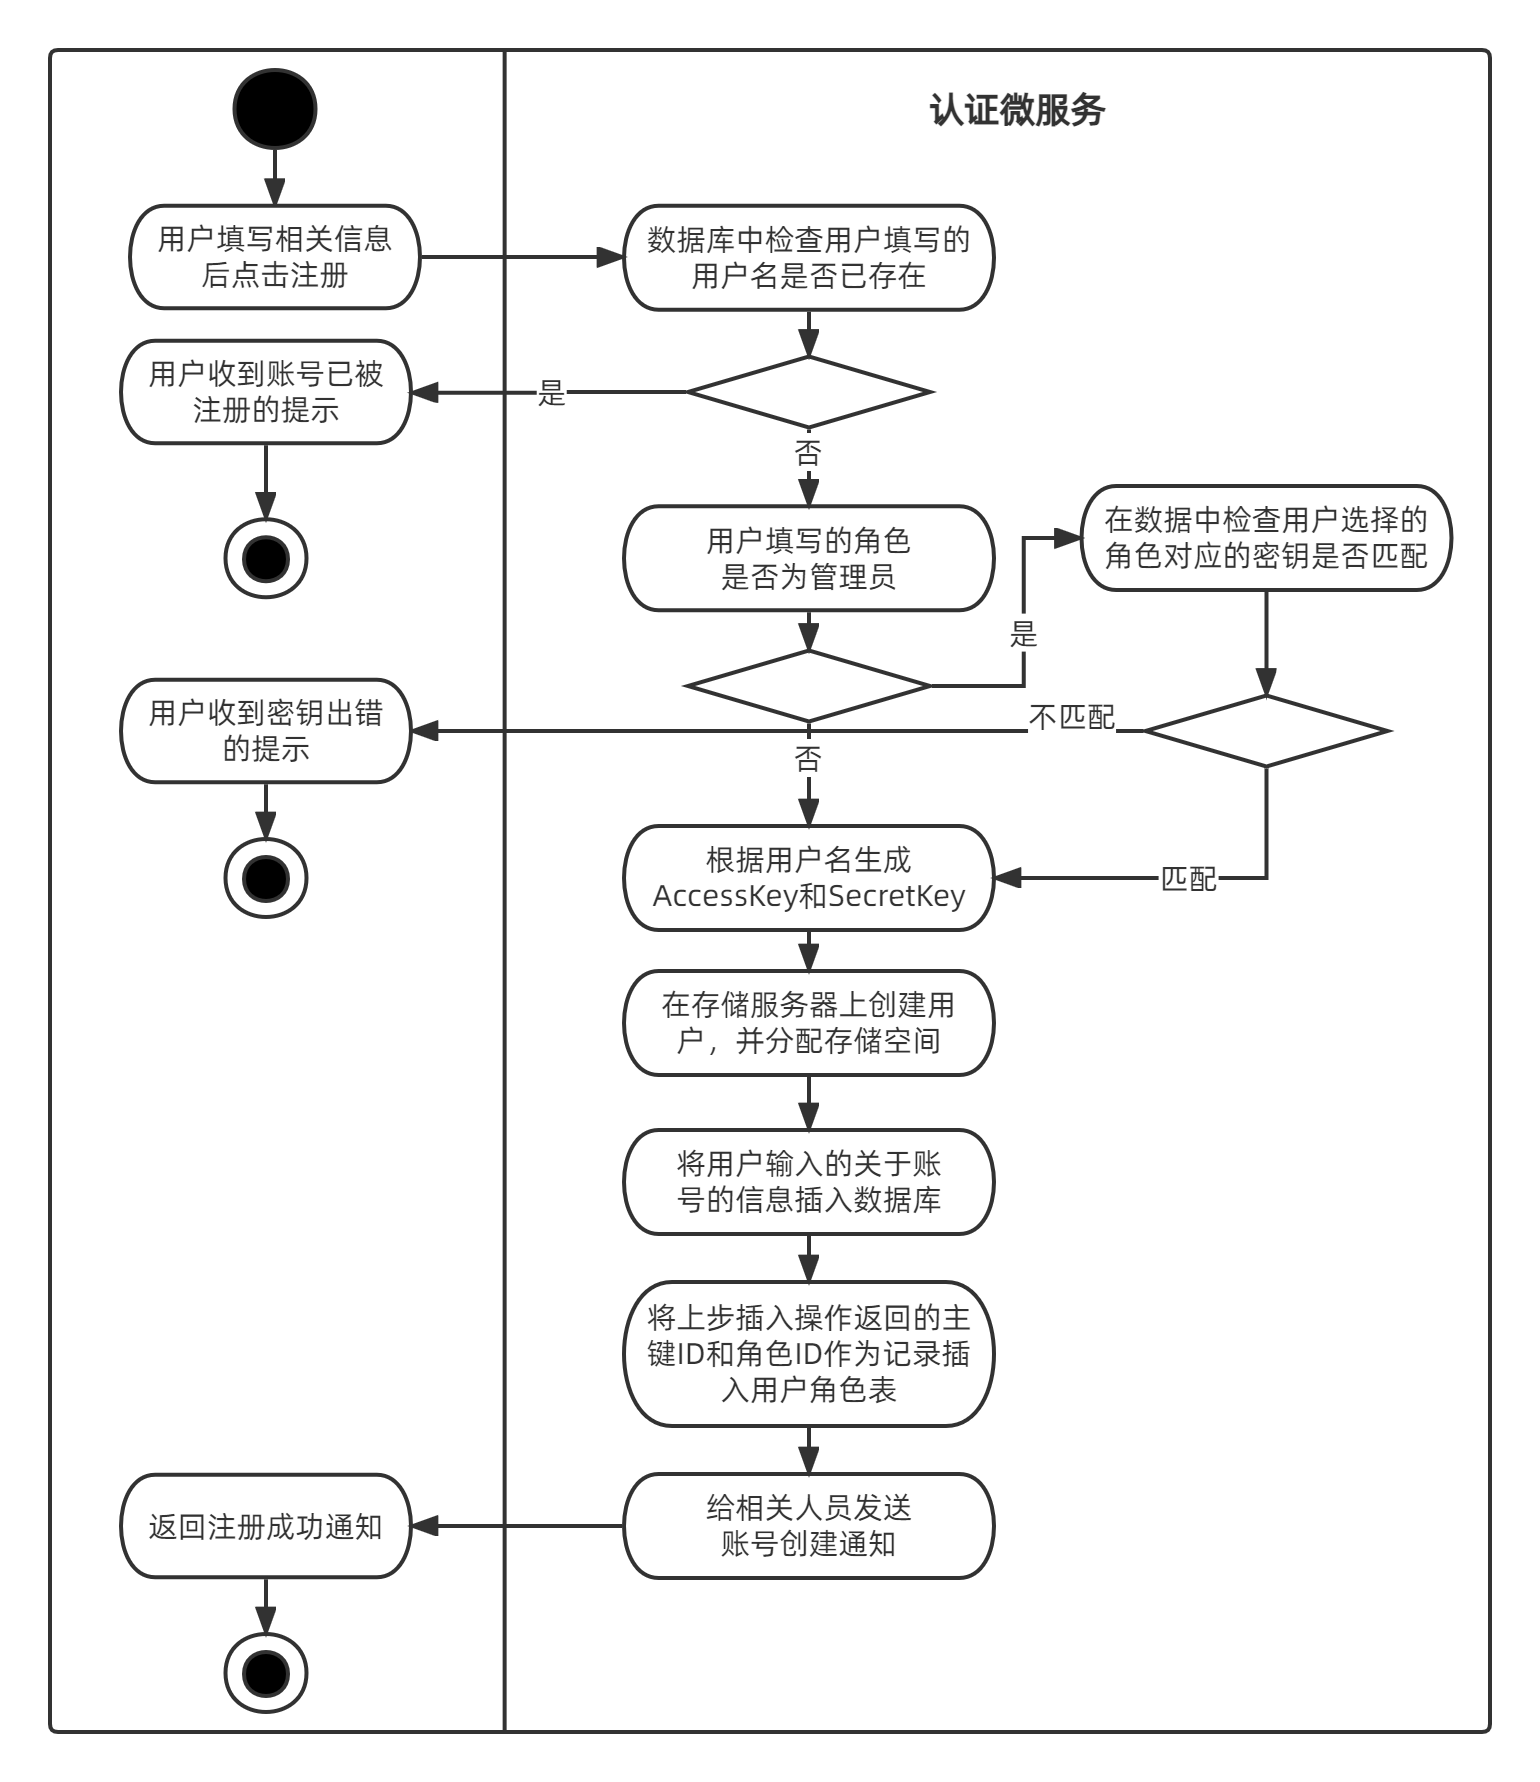
\includegraphics[width=0.7\textwidth]{my_figures/chapter4/用户注册活动图.png}
    \caption{用户注册活动图}
    \label{fig:用户注册活动图}
%     \note{注:图注的内容不宜放到图题中。}
\end{figure}

如果用户所注册的是企业管理员,用户在登录账
号时就必须选择企业管理员的角色,并准确的填写已提前向系统管理员申请的注册密钥,方能进行后续的注册流程,这样做的原因是为了避免外部人员非法获得
管理权限。

如果用户注册的是普通用户,用户在注册时不需要填写密钥,可直接进入后续的注册流程。
用户在注册时需要填写符合要求的用户名和密码,为了提
高账号的安全性,系统对密码的复杂度有一些要求,而且为了满足存储服务器用户名的要求,要求注册使用全英文的用户名。另外,企业管理员用户在注册时还
需要额外填写完整的企业信息和部分个人信息,以供系统管理员审核。


在提交注册信息后,系统首先会检查用户名是否存在,若用户名已存在,则会向前端报错,要求重新输入正确的用户名。在经过校验后,管理员用户或普通用户
都会根据用户名生成相应的AccessKey和 SecretKey,在远程存储服务器上创建对应的管理员用户和普通用户,且会为普通用户分配相应的存储空间。之后,
系统就会把所有用户输入的帐号信息存入数据库的用户列表中,将返回的主键ID与角色ID组成为一条记录,再插入到所有用户角色关联列表中。最后,会向系统
管理员和已注册用户发送用户创建成功的邮件通知,提示用户创建成功。用户注册活动图如图\ref{fig:用户注册活动图}所示。

(2)用户登录



用户在注册成功后会提示进入登录页面,用户填入已经注册成功的账号和密码,并选择角色,即企业管理员或普通用户。在登录请求发出后,系统后端会对用户名、
密码进行校验,以确定账户是否真实存在或密码是否正确。如果用户名不存在,后台会向前端反馈用户名不存在的错误信息。

\begin{figure}[h]
    \centering
    \includegraphics[width=0.7\textwidth]{my_figures/chapter4/用户登录活动图.png}
    \caption{用户登录活动图}
    \label{fig:用户登录活动图}
%     \note{注:图注的内容不宜放到图题中。}
\end{figure}

对于密码的校验,系统则是通过选择的hash函数对密码进行hash计算后与数据库系统中的密码进行对比,这是因为数据库系统中保存的都是已经利用hash处理过
的密码,一旦实现了配对,将通过相应的方法得到token,否则将由前端反馈密码错误的信息。密码认证活动图如图\ref{fig:用户登录活动图}所示。


(3)身份认证

JSON Web Token(JWT)是一种开放规范,旨在可靠地传递JSON数据。它定义了一种新的数据格式,由Header、Payload和Signature这三部分组成,这些部分的分隔符是英文句点。
Header由token形式和所使用的签名技术两个部分组成。Payload是JWT的基本组成部分,用于存储业务信息,它包含七个默认字段,例如:Payload发行人、过期日期、JWT编号等,
供开发人员使用。
\begin{figure}[htb]
    \centering
    \includegraphics[width=0.7\textwidth]{my_figures/chapter4/身份认证活动图.png}
    \caption{身份认证活动图}
    \label{fig:身份认证活动图}
%     \note{注:图注的内容不宜放到图题中。}
\end{figure}
此外,开发人员还可以添加自定义字段,如角色信息和时间戳信息等。由于这部分数据未经过严格的保密处理,不能将整个系统的加密数据建立在此部分。实际上,Signature部分的功
能可以防止该令牌被篡改,而JWT的Header部分则记录了使用的加密算法。颁发令牌活动图如图\ref{fig:身份认证活动图}所示。


% (4)认证令牌

% 这个过程主要是为了避免 token被篡改,篡改后的 token无法通过验证。之后,系统会对token在第二部分中的时间戳做出判断,重点就是检测时间戳有没有过期,
% 一旦时间戳已经过期,那么用户就必须重新登录并再次申请token。过期日期也可以由开发人员灵活设定,但过期日期需要设定的适当,太长或太短都会存在优点和缺点。
% 若将过期日期设定的太短,优点是安全性比较好,即使 token泄漏,token也会马上失效;缺点是用户需要在很短的时间内反复重新登录,体验极差。如果过期日期设
% 定的较长,好处是客户不必频繁重复登录,能长期保持注册状态;坏处是不法分子有了更多的时间进行非法操作。通过认证后,网关会将消息转发给其他各个微服务
% 模块,用户可进行需要的操作。认证令牌活动图如图\ref{fig:认证令牌活动图}所示。

% \begin{figure}[htb]
%     \centering
%     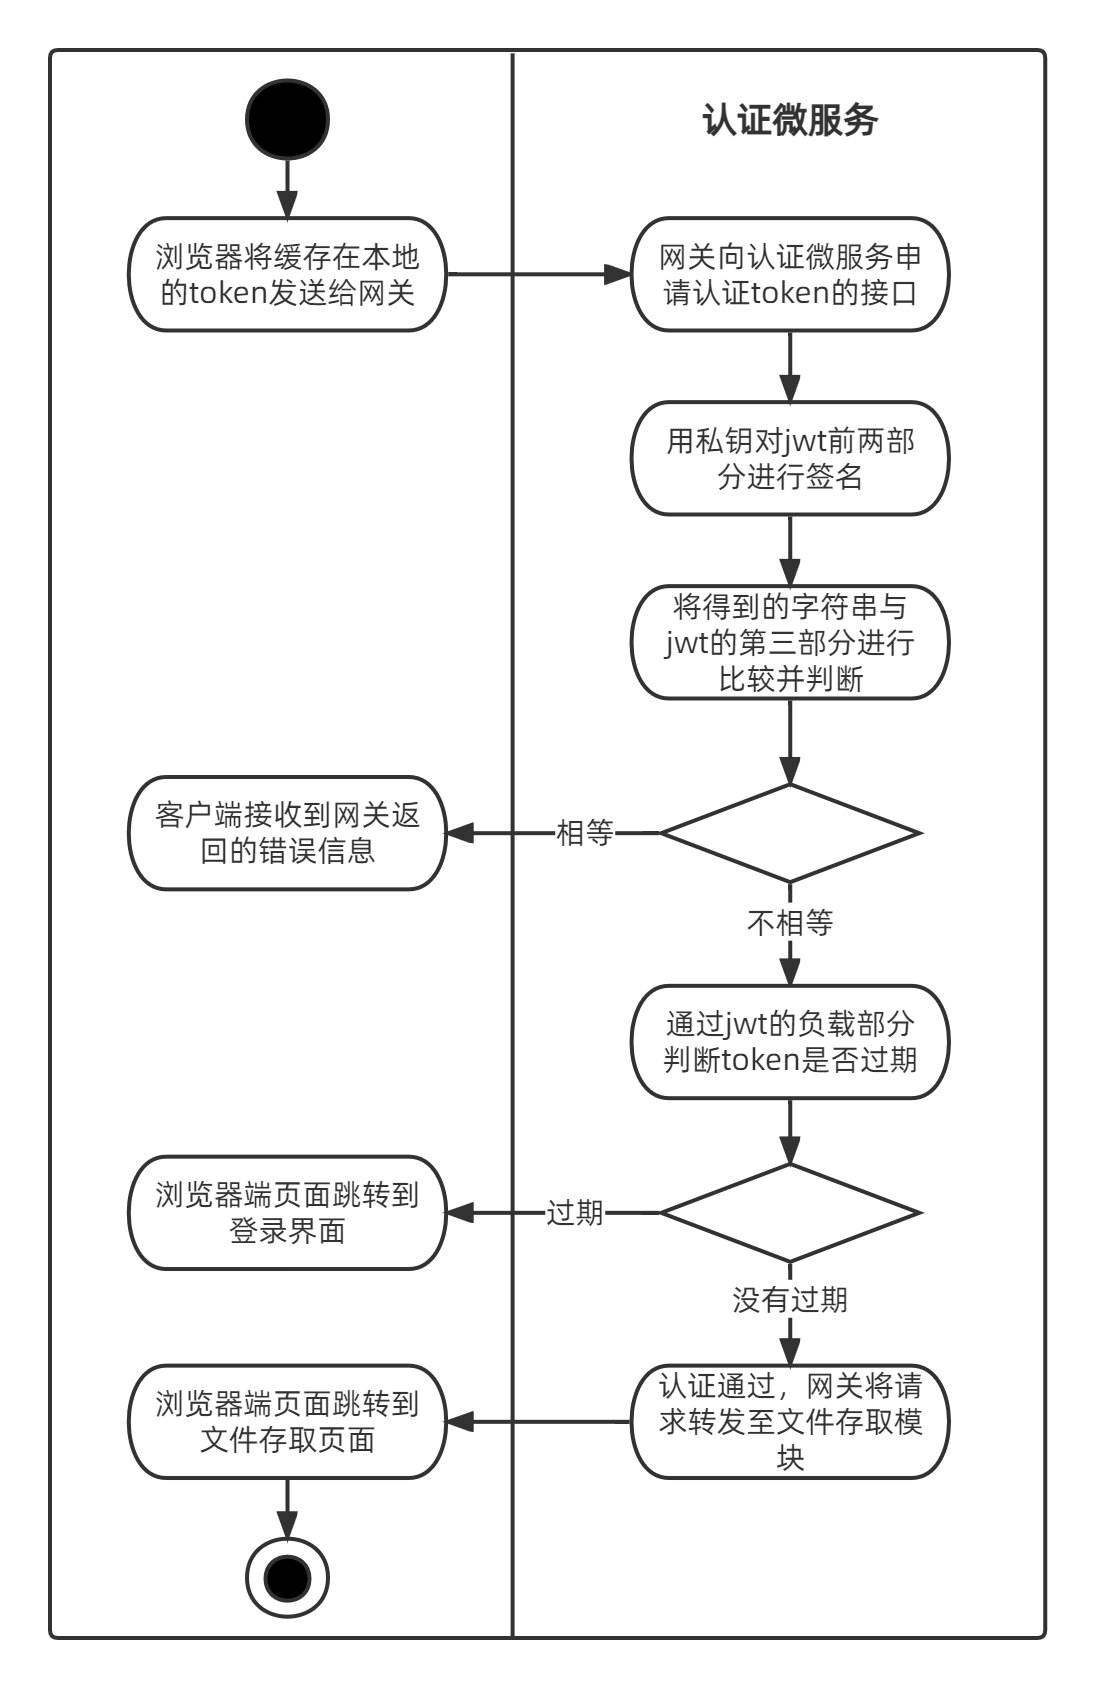
\includegraphics[width=0.7\textwidth]{my_figures/chapter4/认证令牌活动图.png}
%     \caption{认证令牌活动图}
%     \label{fig:认证令牌活动图}
% %     \note{注:图注的内容不宜放到图题中。}
% \end{figure}

\subsection{权限控制模块}

\begin{figure}[h]
    \centering
    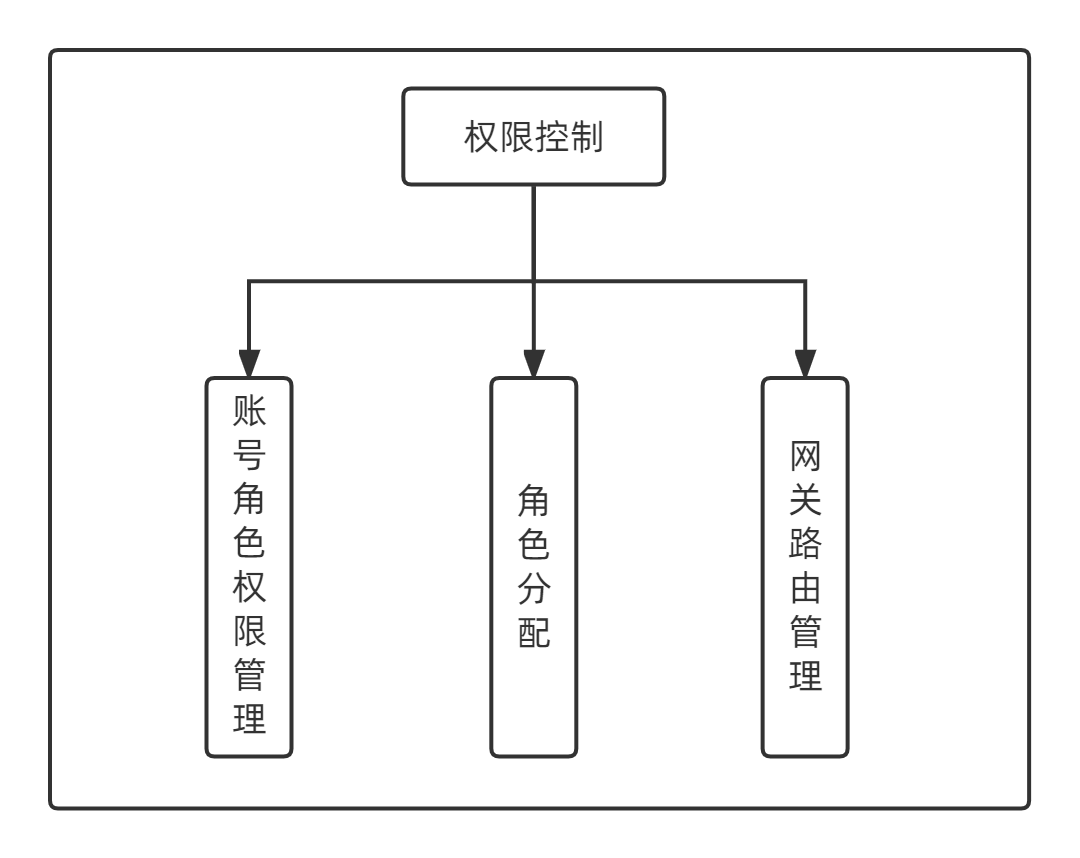
\includegraphics[width=0.5\textwidth]{my_figures/chapter4/权限控制模块功能结构图.png}
    \caption{权限控制模块功能结构图}
    \label{fig:权限控制模块功能结构图}
%     \note{注:图注的内容不宜放到图题中。}
\end{figure}

权限控制模块的主要功能是系统管理员用来管理的角色、权限和网关路由,以及控制整个微服务的入口。

权限控制模块是系统架构中重要的一部分,它主要由三个子功能模块组成:权限管理、角色管理和网关鉴权。其中,权限管理和角色管理负责对角色和权限的信息进行管理和分配,以确
保用户能够访问所需的资源,而网关鉴权则主要通过各种安全方面的校验,为整个系统提供保护。在此过程中,操作系统会将网关的所有接口作为唯一的入口,确保所有的请求都经过安
全筛选。这样,就可以有效地保护系统不被未经授权的人员或攻击者访问,确保系统的安全性和稳定性。权限控制模块的功能结构图如图\ref{fig:权限控制模块功能结构图}所示。




(1)权限管理

权限管理子模块是整个权限控制模块中的一个重要组成部分。该子模块负责权限的创建、删除、修改、查询和分配等管理工作。在系统中,权限实际上对应于每一个功能接口,即用户是
否有权限访问某个功能接口,进行相关操作。拥有某接口的访问权限本质上就是拥有其访问路径,角色的权限列表中存储的内容就是该角色可访问的路径。权限分配的过程就是将权限与
角色进行绑定。在角色的权限列表中加入某接口的访问路径,则该角色拥有了访问该功能接口的权限。因此,拥有该角色的用户同样也具备该权限,从而可以执行相应的操作。这种方式
可以有效地限制用户权限,保证系统的安全性和稳定性。由于权限管理的逻辑与角色管理十分相似,所以它们的活动图也基本相同,故此处可参考角色管理的活动图\ref{fig:角色管理活动图}。

% 权限管理活动图如图\ref{fig:权限管理活动图}所示。

% \begin{figure}[h]
%     \centering
%     \includegraphics[width=0.7\textwidth]{my_figures/chapter4/权限管理活动图.png}
%     \caption{权限管理活动图}
%     \label{fig:权限管理活动图}
% %     \note{注:图注的内容不宜放到图题中。}
% \end{figure}

(2)角色管理

角色管理子模块主要包含角色查询和分配功能。该系统默认只支持系统管理员、企业管理员和普通用户三种角色,因此不支持新角色的创建、修改和删除系统默认角色。角色分配系统负
责将用户、权限和角色进行绑定,将角色分配给用户相当于为员工设置职务,将权限与角色进行绑定相当于为职位授予相应的权限。为保护这两个关系,系统设计了用户角色关联表和角
色权限关联表。用户角色关联表记录包含用户ID和角色ID两部分,角色权限关联表记录则包含角色ID和权限ID两部分。系统管理员可能会同时将角色与用户和权限进行绑定或解绑。在实
现时,必须实施数据库事务管理,以保护这些关联关系。如果在事务处理过程中出现错误,可以及时地对操作进行回滚,确保数据的完整性。
角色管理活动图如图\ref{fig:角色管理活动图}所示。

\begin{figure}[h]
    \centering
    \includegraphics[width=0.7\textwidth]{my_figures/chapter4/角色管理活动图.png}
    \caption{角色管理活动图}
    \label{fig:角色管理活动图}
%     \note{注:图注的内容不宜放到图题中。}
\end{figure}

(3)网关鉴权

在微服务架构中,请求转发是指接收到一个请求后,将其转发给下一个处理节点。当系统收到一个操作请求时,会按照设定的路由信息转发到指定的微服务,根据
系统微服务的划分一共设置了五个网关路由项,路由项分别由不同的前缀字段组成,注册认证微服务对应的路由项为/Oauth,权限控制微服务对应的路由项为
/Perm,策略控制微服务对应的路由项为/policyweb,文件存取微服务对应的路由项为/fileweb,系统监控微服务对应的路由项为/systemweb。

\begin{figure}[h]
    \centering
    \includegraphics[width=0.7\textwidth]{my_figures/chapter4/网关鉴权活动图.png}
    \caption{网关鉴权活动图}
    \label{fig:网关鉴权活动图}
%     \note{注:图注的内容不宜放到图题中。}
\end{figure}

系统将用户请求中的前缀与路由项进行对比以决定转发给对应的微服务,如果是转发至策略控制、文件存取和系统监控这三个微服务的请求,系统会使用过滤器对
这些请求进行过滤。网关会在过滤器中调用认证令牌子模块的接口来检查 token 的正确性,如果 token 检查通过,则会调用权限管理模块中的接口。权限管理
模块根据token中的用户名来获取用户的权限列表,该权限列表中包含了用户可访问的路径。然后,过滤器会查找用户权限列表来判断用户请求中的URI是否存在
于该列表中。如果该路径存在,则说明用户拥有访问该接口的权限,否则没有访问权限。在没有权限的情况下,过滤器会向前端返回错误信息。这种设计保证了
只有具有相应权限的用户才能够访问特定的接口,从而提高了系统的安全性。网关鉴权活动图如图\ref{fig:网关鉴权活动图}所示。



\subsection{策略控制模块}

策略控制模块主要负责对注册在存储服务器上的用户、分组和访问策略进行管理。策略控制模块主要包含三个子模块,分别是用户管理子模块、策略管理子模块和
策略分配子模块。用户管理子模块主要负责对存储用户的相关数据信息进行管理,策略管理子模块主要负责对访问策
略的相关数据信息进行管理,策略分配主要负责将策略与用户、策略与分组进行关联,处理这三者之间的分配关系。策略控制模块功能结构如图\ref{fig:策略控制模块功能结构图}
所示。

\begin{figure}[htb]
    \centering
    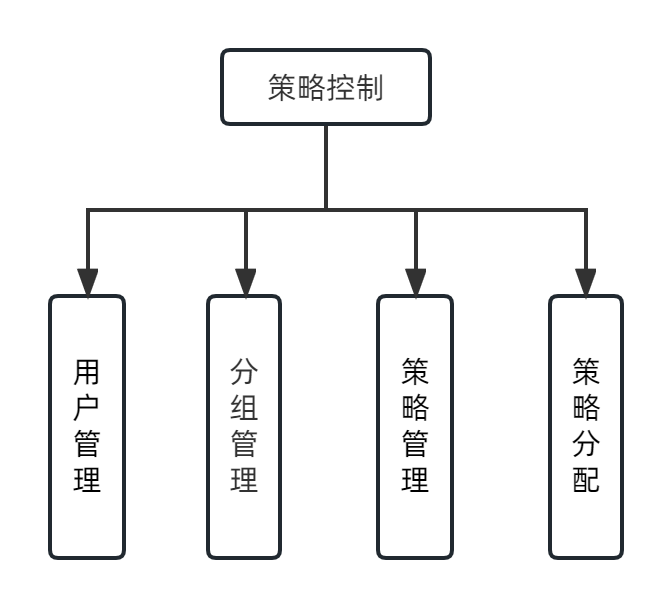
\includegraphics[width=0.5\textwidth]{my_figures/chapter4/策略控制模块功能结构图.png}
    \caption{策略控制模块功能结构图}
    \label{fig:策略控制模块功能结构图}
%     \note{注:图注的内容不宜放到图题中。}
\end{figure}

(1) 用户管理

用户管理主要负责对用户账号信息进行数据管理。管理员可以通过该模块对用户进行增加、删除、修改、查看和禁用等操作。用户的信息包括用户名、密码、邮箱、申请容量、已用容量
等项内容。当需要创建新用户时,管理员需要在界面上输入用户信息,并且对用户密码进行加密存储,最后将用户信息保存到数据库中。此外,与此同时,在对象存储服务器上也会创建
一个同名的账户。用户信息中的申请容量和已用容量等内容都是通过存储服务器获取的。因此,当管理员进行修改、删除、查询等操作时,都需要同时从数据库和存储服务器中获取数据
。这样才能保证用户账号信息的实时性和准确性。用户的权限由其所属的角色决定,而角色和权限则是在权限控制模块中进行绑定的。在新创建用户时,管理员可以为其选择所属的角色
以确定其所拥有的权限。这样做可以保证权限授权的便捷性和灵活性,从而有效地简化了进行权限控制的工作流程。

当系统进行用户管理的相关操作时,相关操作请求会调用网关鉴权微服务接口,查找用户权限列表来判断用户请求中的URI是否存在于该列表中。如果该路径
存在,则说明用户拥有访问该接口的权限,否则没有访问权限。如果没有访问权限,用户会在前端页面上收到无访问权限的提示,如果有权限,系统会与存储服务
客户端AliIO-Cli建立连接,调用客户端AliIO-Cli提供的用户管理相关API接口,由客户端将请求发送给存储服务器节点。存储服务器节点将完成状态或查询信息反馈给
客户端AliIO-Cli,然后系统调用AliIO-Cli提供的相关API取回状态或查询信息,并在前端页面进行展示。用户管理活动图如图\ref{fig:用户管理活动图}所示。

\begin{figure}[htb]
    \centering
    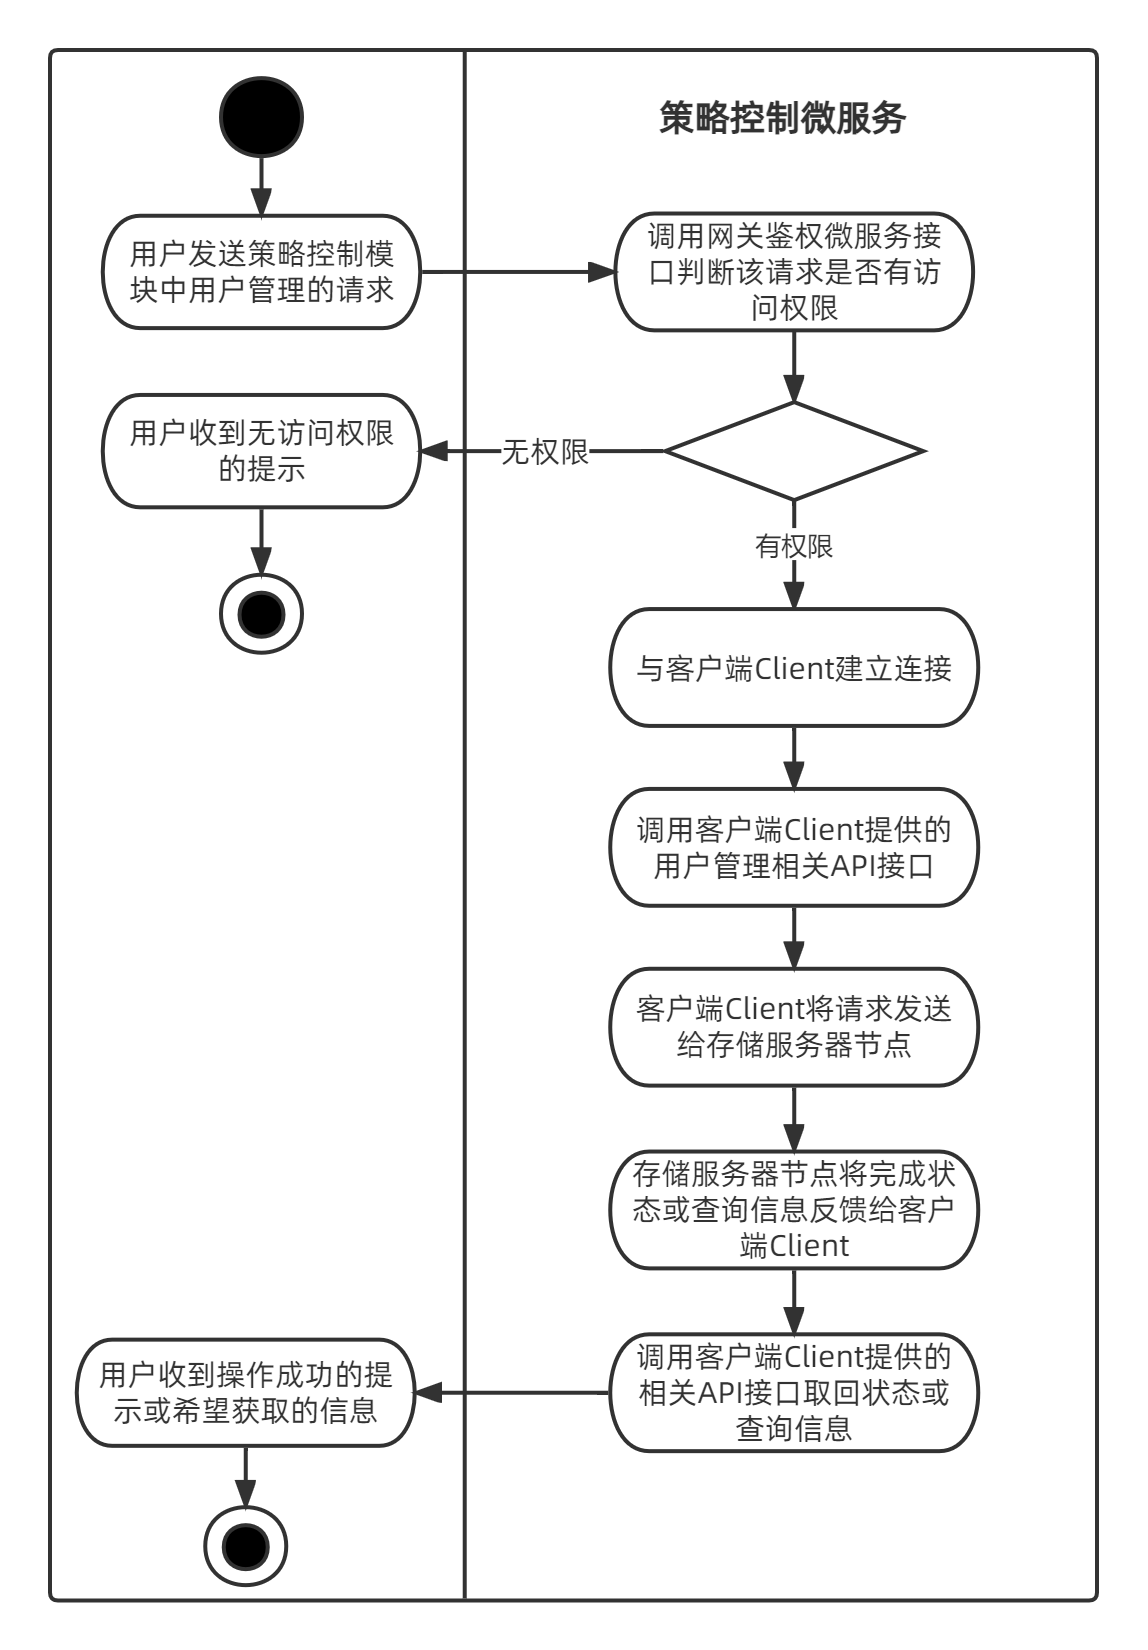
\includegraphics[width=0.7\textwidth]{my_figures/chapter4/用户管理活动图.png}
    \caption{用户管理活动图}
    \label{fig:用户管理活动图}
%     \note{注:图注的内容不宜放到图题中。}
\end{figure}

% (2) 分组管理

% 分组管理主要负责存储服务器分组信息进行数据管理。可以对分组进行增加、删除、修改、查看和禁用操作。存储服务器分组主要包括分组名称、访问策略、是否禁用和创建时间
% 等信息。当系统发出对分组管理模块的使用申请时,首先会使用网关鉴权微服务进行鉴权,如果没授权,会向前端反馈错误的信息,如果有授权,则与客户端AliIO-Cli建立连接,并
% 调用客户端AliIO-Cli提供的API接口,由客户端AliIO-Cli将请求发送给存储服务器节点,待存储服务器处理结束后,会将完成状态或查询信息反馈给客户端AliIO-Cli,管理系统调用客户
% 端AliIO-Cli提供的API取回状态或查询信息,并反馈给前端。分组管理活动图与用户管理活动图十分类似,可参考用户管理活动图\ref{fig:用户管理活动图}。

% \begin{figure}[htb]
%     \centering
%     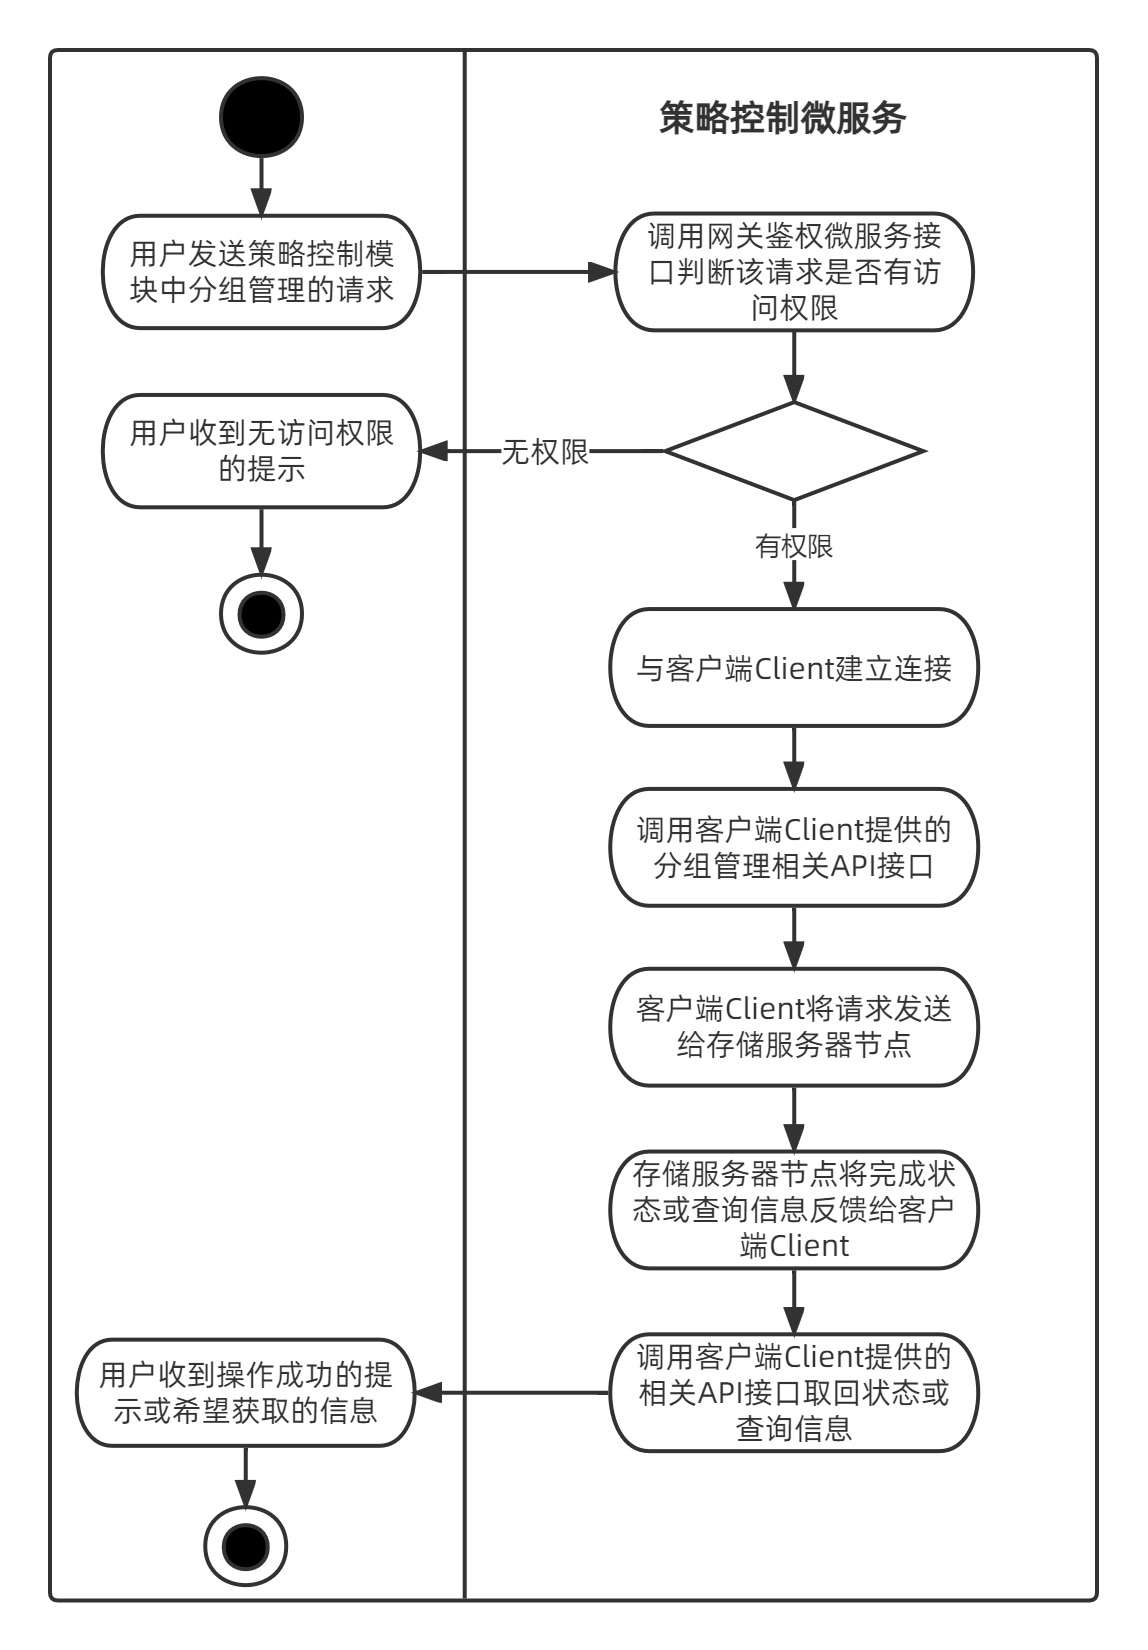
\includegraphics[width=0.8\textwidth]{my_figures/chapter4/分组管理活动图.png}
%     \caption{分组管理活动图}
%     \label{fig:分组管理活动图}
% %     \note{注:图注的内容不宜放到图题中。}
% \end{figure}

(2) 策略管理

策略管理主要负责存储服务器访问策略信息进行数据管理。可以对策略进行增加、删除、修改、查看操作。访问策略主要是针对用户和分组在访问其他用户的Bucket和文件时进行
权限限制,系统已经内置了几种常用的访问策略, 系统中的策略主要分为Bucket访问策略和用户访问策略。
\begin{figure}[htb]
    \centering
    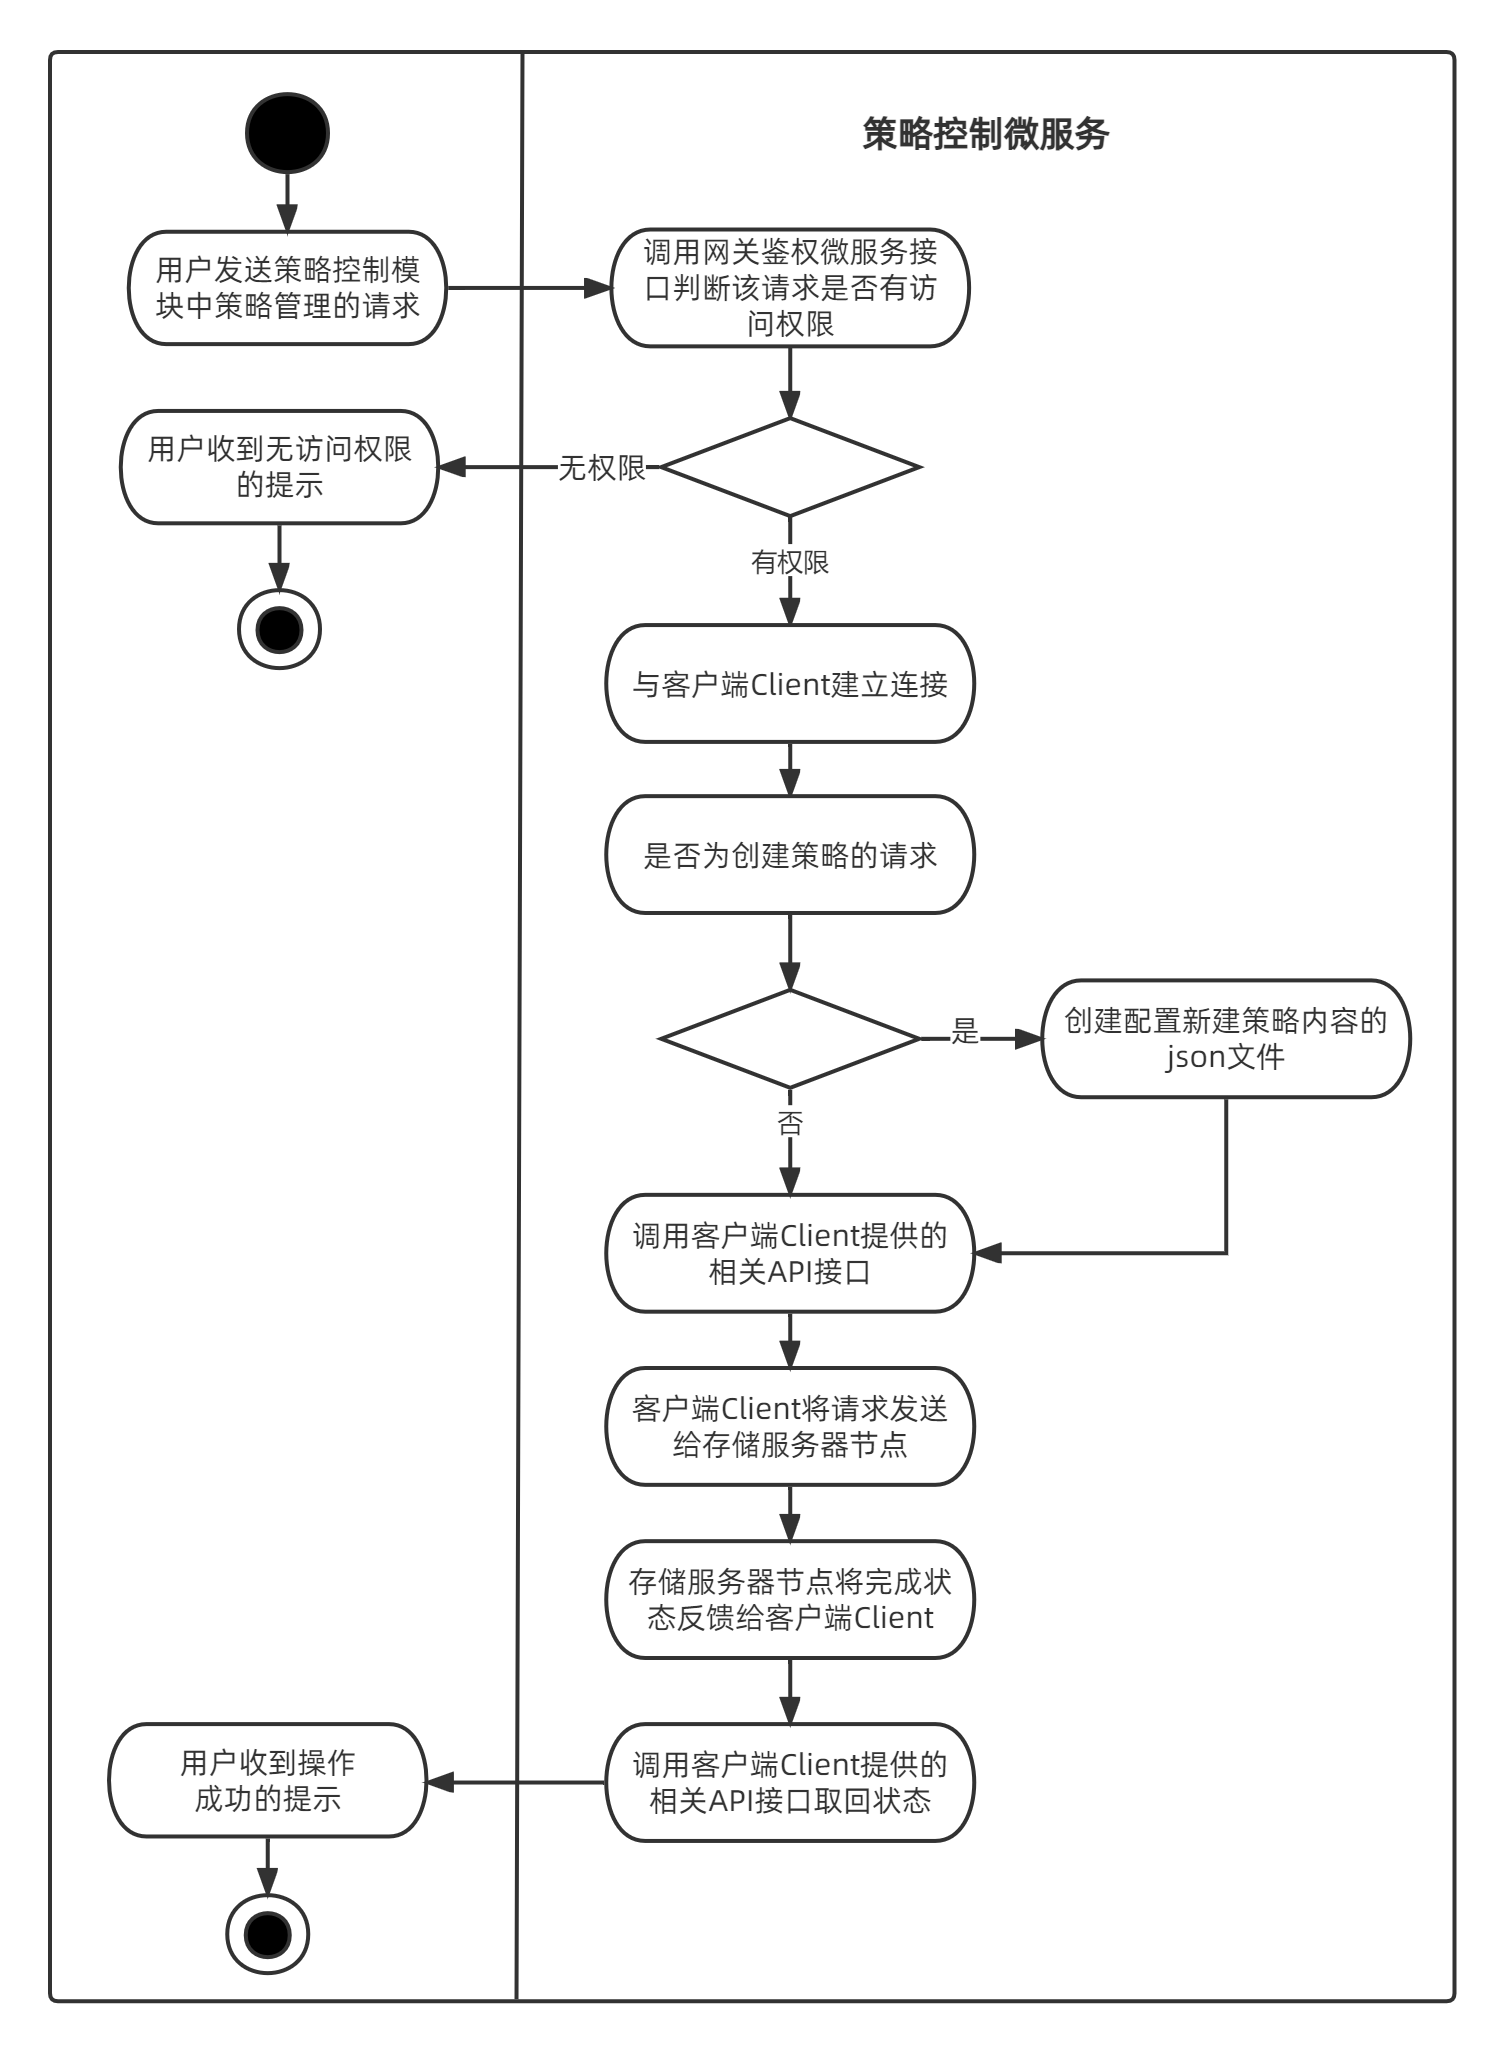
\includegraphics[width=0.7\textwidth]{my_figures/chapter4/策略管理活动图.png}
    \caption{策略管理活动图}
    \label{fig:策略管理活动图}
%     \note{注:图注的内容不宜放到图题中。}
\end{figure} 
Bucket访问策略主要有public、custom和private
三种,系统内置的用户访问策略主要有五种,分别是控制台管理员(consoleAdmin)策略、诊断(diagnostics)策略、只读(readonly)策略、
读写(readwrite)策略和只写(writeonly)策略。

当设置Bucket的使用方式是public后,用户必须不通过任何验证才能进行使用资源;当设置Bucket的访问
方式是custom后,Bucket的最终访问策略由具体的用户访问策略决定,用户访问策略可以是系统内定的策略,如只读(readonly)策略、读写(readwrite)策
略和只写(writeonly)策略,也可以是自定义的访问策略;当设置Bucket的访问策略为private时,用户未经授权不能进行任何操作,所有用户访问策略失效。
因此,Bucket的访问策略权限要大于用户访问策略。

当管理员在执行策略管理的相关操作时,如果是创建新的策略,那么管理员需要配置相关的策略模板文件,该文件包含新策略的实际内容。该文件主要含有Version、
Statement、Effect、Principal、Action、Resource等配置项,管理员可根据需要自定义该文件的内容。当删除某个自定义的策略时,如果
有用户或分组正在使用该策略,则删除该策略后,用户或分组的策略会自动变为默认的策略。策略管理活动图如图\ref{fig:策略管理活动图}所示。

(3) 策略分配




策略分配主要负责将预定义的策略分配给特定的用户或用户组,以控制他们对存储桶和对象的访问权限。当管理员登录到管控平台,进入策略管理页面,管理员
选择一个或多个用户或用户组,然后将预定义的策略分配给他们。

\begin{figure}[h]
    \centering
    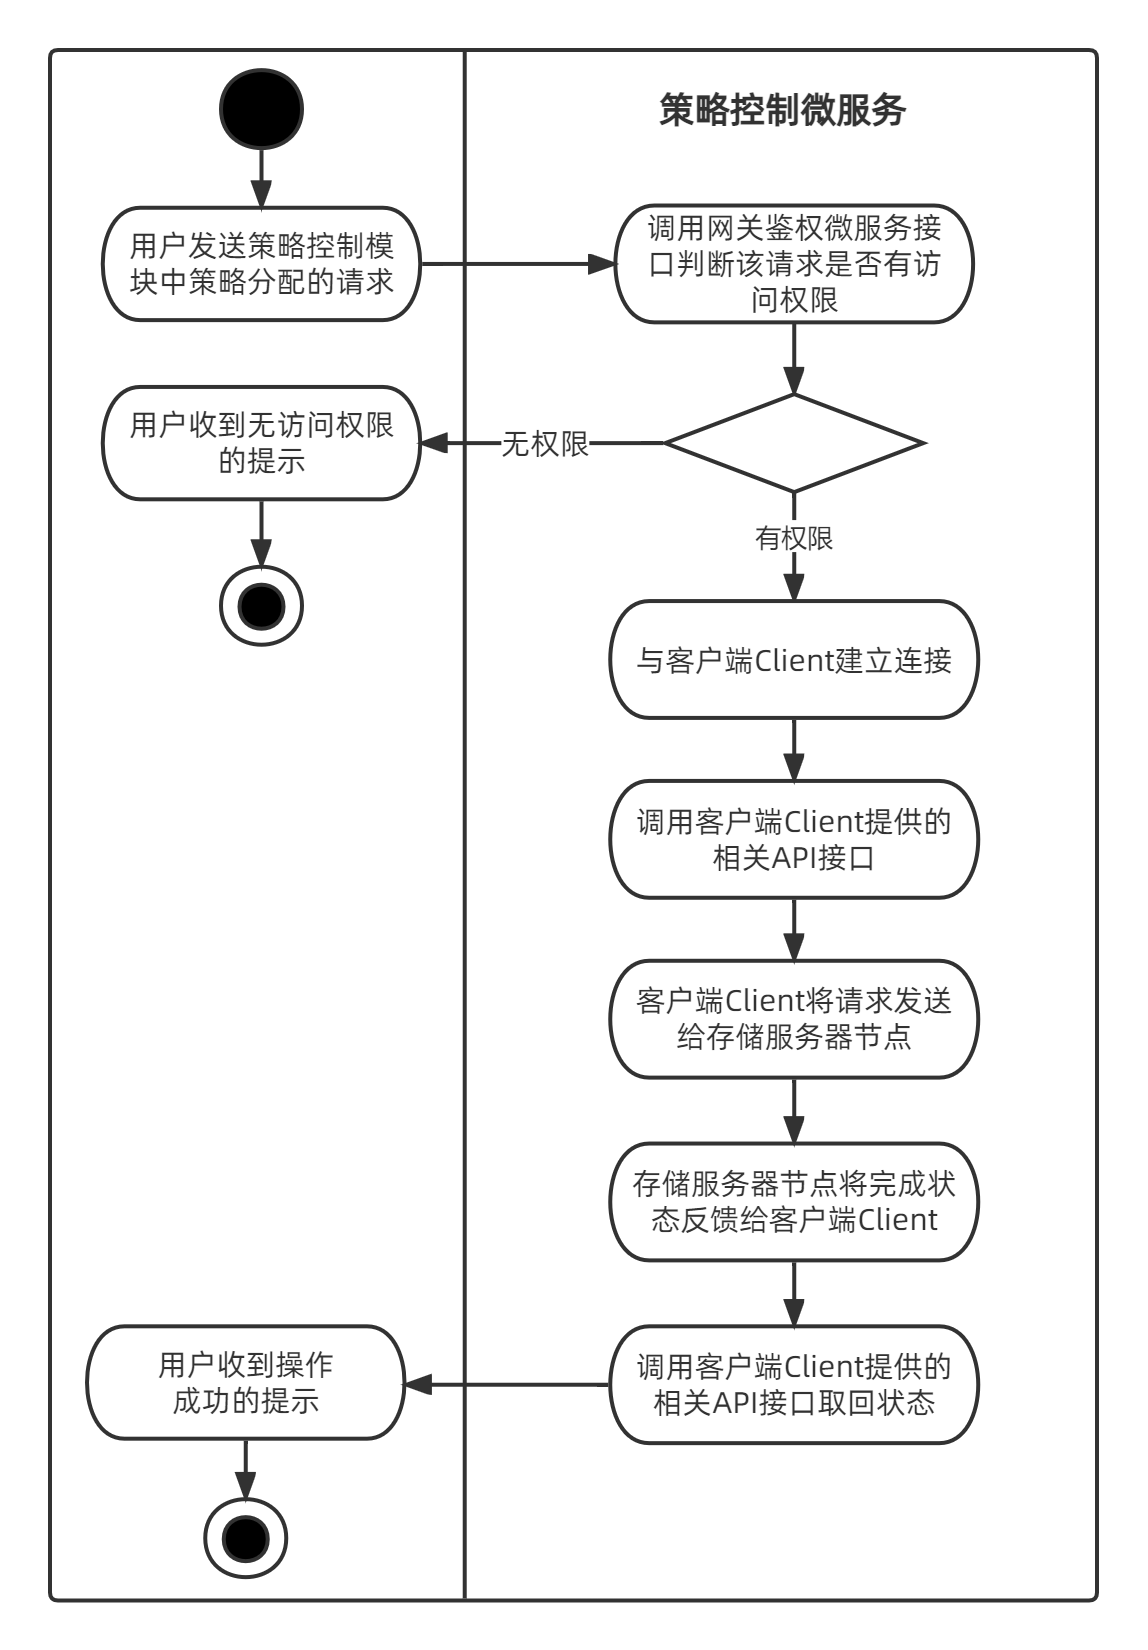
\includegraphics[width=0.7\textwidth]{my_figures/chapter4/策略分配活动图.png}
    \caption{策略分配活动图}
    \label{fig:策略分配活动图}
%     \note{注:图注的内容不宜放到图题中。}
\end{figure}

为了更加精细地管控存储系统的访问权限,管理员可以在分配策略时设置各种参数,如存储桶的访问权限、对象的访问权限以及访问时间等。一旦管理员保存了策略,管控平台会自动将
策略授权信息同步到后端的对象存储系统中。此外,管理员还可以同时向用户或用户组分配策略。如果一个用户属于某个分组,且分组策略与用户策略不同,则管理员需对用户的策略进
行升级,以满足分组策略的要求。如果分组策略不如用户策略严格,则用户可以继续使用其原有的策略,以保持其现有的权限状态。策略分配活动图如图\ref{fig:策略分配活动图}所
示。



\subsection{文件存取模块}

% 文件存储模块是本系统最核心的模块,也是普通用户访问最频繁的模块,该模块主要分为四个子模块,分别是桶管理子模块、文件上传子模块、文件下载子模块和文件删除子模块。
% 文件存取模块功能结构图如图\ref{fig:文件存取模块功能结构图}所示。
\begin{figure}[h]
    \centering
    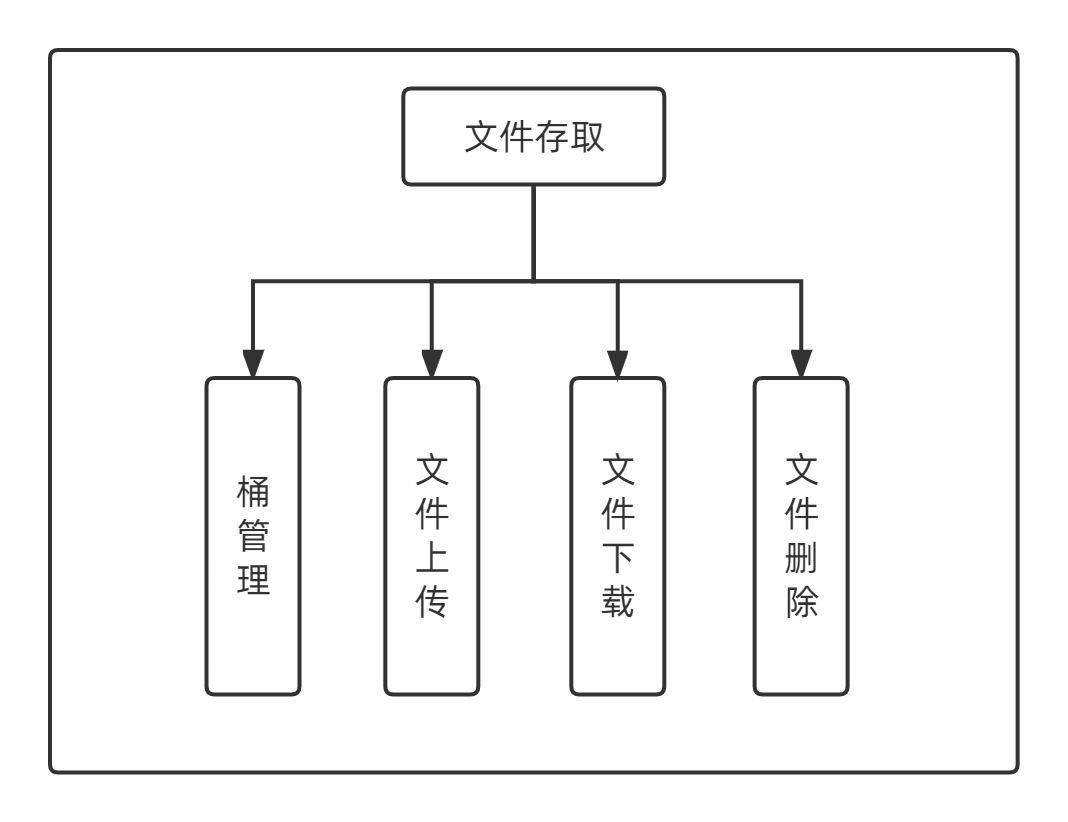
\includegraphics[width=0.5\textwidth]{my_figures/chapter4/文件存取模块功能结构图.png}
    \caption{文件存取模块功能结构图}
    \label{fig:文件存取模块功能结构图}
%     \note{注:图注的内容不宜放到图题中。}
\end{figure}

文件存储模块是本系列中最基础的功能,同时也是普通用户使用最频繁的功能,该模块主要包括了三大子模块,分别为桶管理子模块、
文件上传子模块和文件下载子模块。文件存取模块功能的结构图如图\ref{fig:文件存取模块功能结构图}所示。



(1) 桶管理



桶管理模块是对用户存储桶的管理功能的主要模块。其中包括创建、删除、修改桶属性、查看桶列表以及查看桶属性等操作。然而在进行这些操作时,前提条件是用户必须拥有相应的访
问策略。例如,如果用户只有针对某个桶的只读访问策略,则只能查看该桶,无法进行其他的修改、删除等操作。
\begin{figure}[htb]
    \centering
    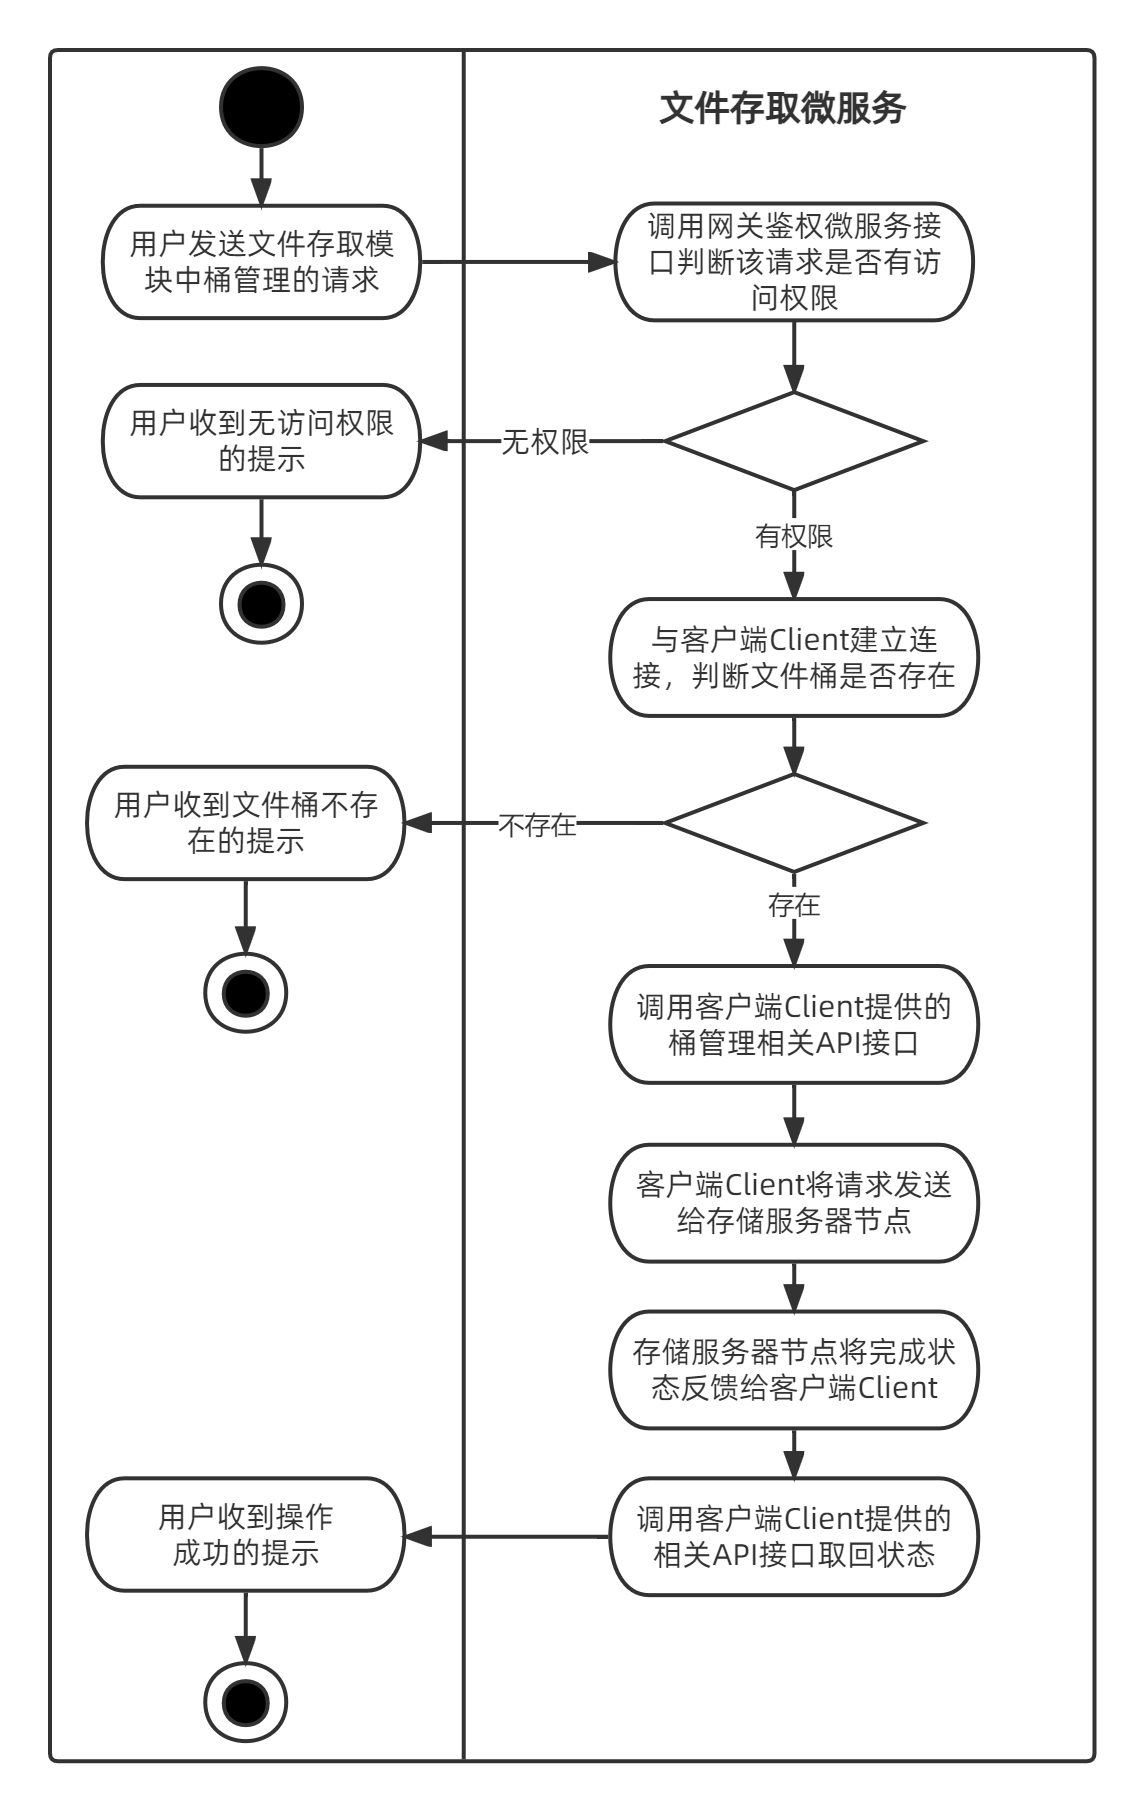
\includegraphics[width=0.7\textwidth]{my_figures/chapter4/桶管理活动图.png}
    \caption{桶管理活动图}
    \label{fig:桶管理活动图}
%     \note{注:图注的内容不宜放到图题中。}
\end{figure}

在系统中创建新的桶时,用户需要填写唯一的名称、访问权限、存储类型以及其他属性。用户需要根据需求来确定桶的存储空间、容量、生命周期等设置,让其可以满足后续的文件上传、
访问以及管理需求。进行删除操作时,需要用户先确认以确保不会误删桶内的所有文件。删除桶时,则需先删除桶内的所有文件,之后再执行删除桶的操作。此外,用户还可以修改桶的
各种属性,例如桶的名称、访问权限、存储类型、生命周期等。在修改桶属性时,用户需要注意,某些属性的修改可能会影响到桶内已有的文件,因此需要慎重处理。

此外,用户还可以查看桶列表以及桶的属性,并基于桶名称、存储区域等条件进行搜索与过滤,方便快速定位目标桶。用户可以查看指定桶的详细属性信息,其中包含桶名称、访问权限、生命周期、当前使用量、文件数量等。此外,还支持用户查看桶内的文件列表、访问日志等信息,以便于快速监控和管理。
当用户执行上述除创建以外的操作时,需要先判断桶是否存在。如果桶不存在,前端页面将会显示文件不存在的提示。如果存在,则会继续跟对象存储系统服务器进行交互。
桶管理活动图如图\ref{fig:桶管理活动图}所示。




(2) 文件上传

\begin{figure}[htb]
    \centering
    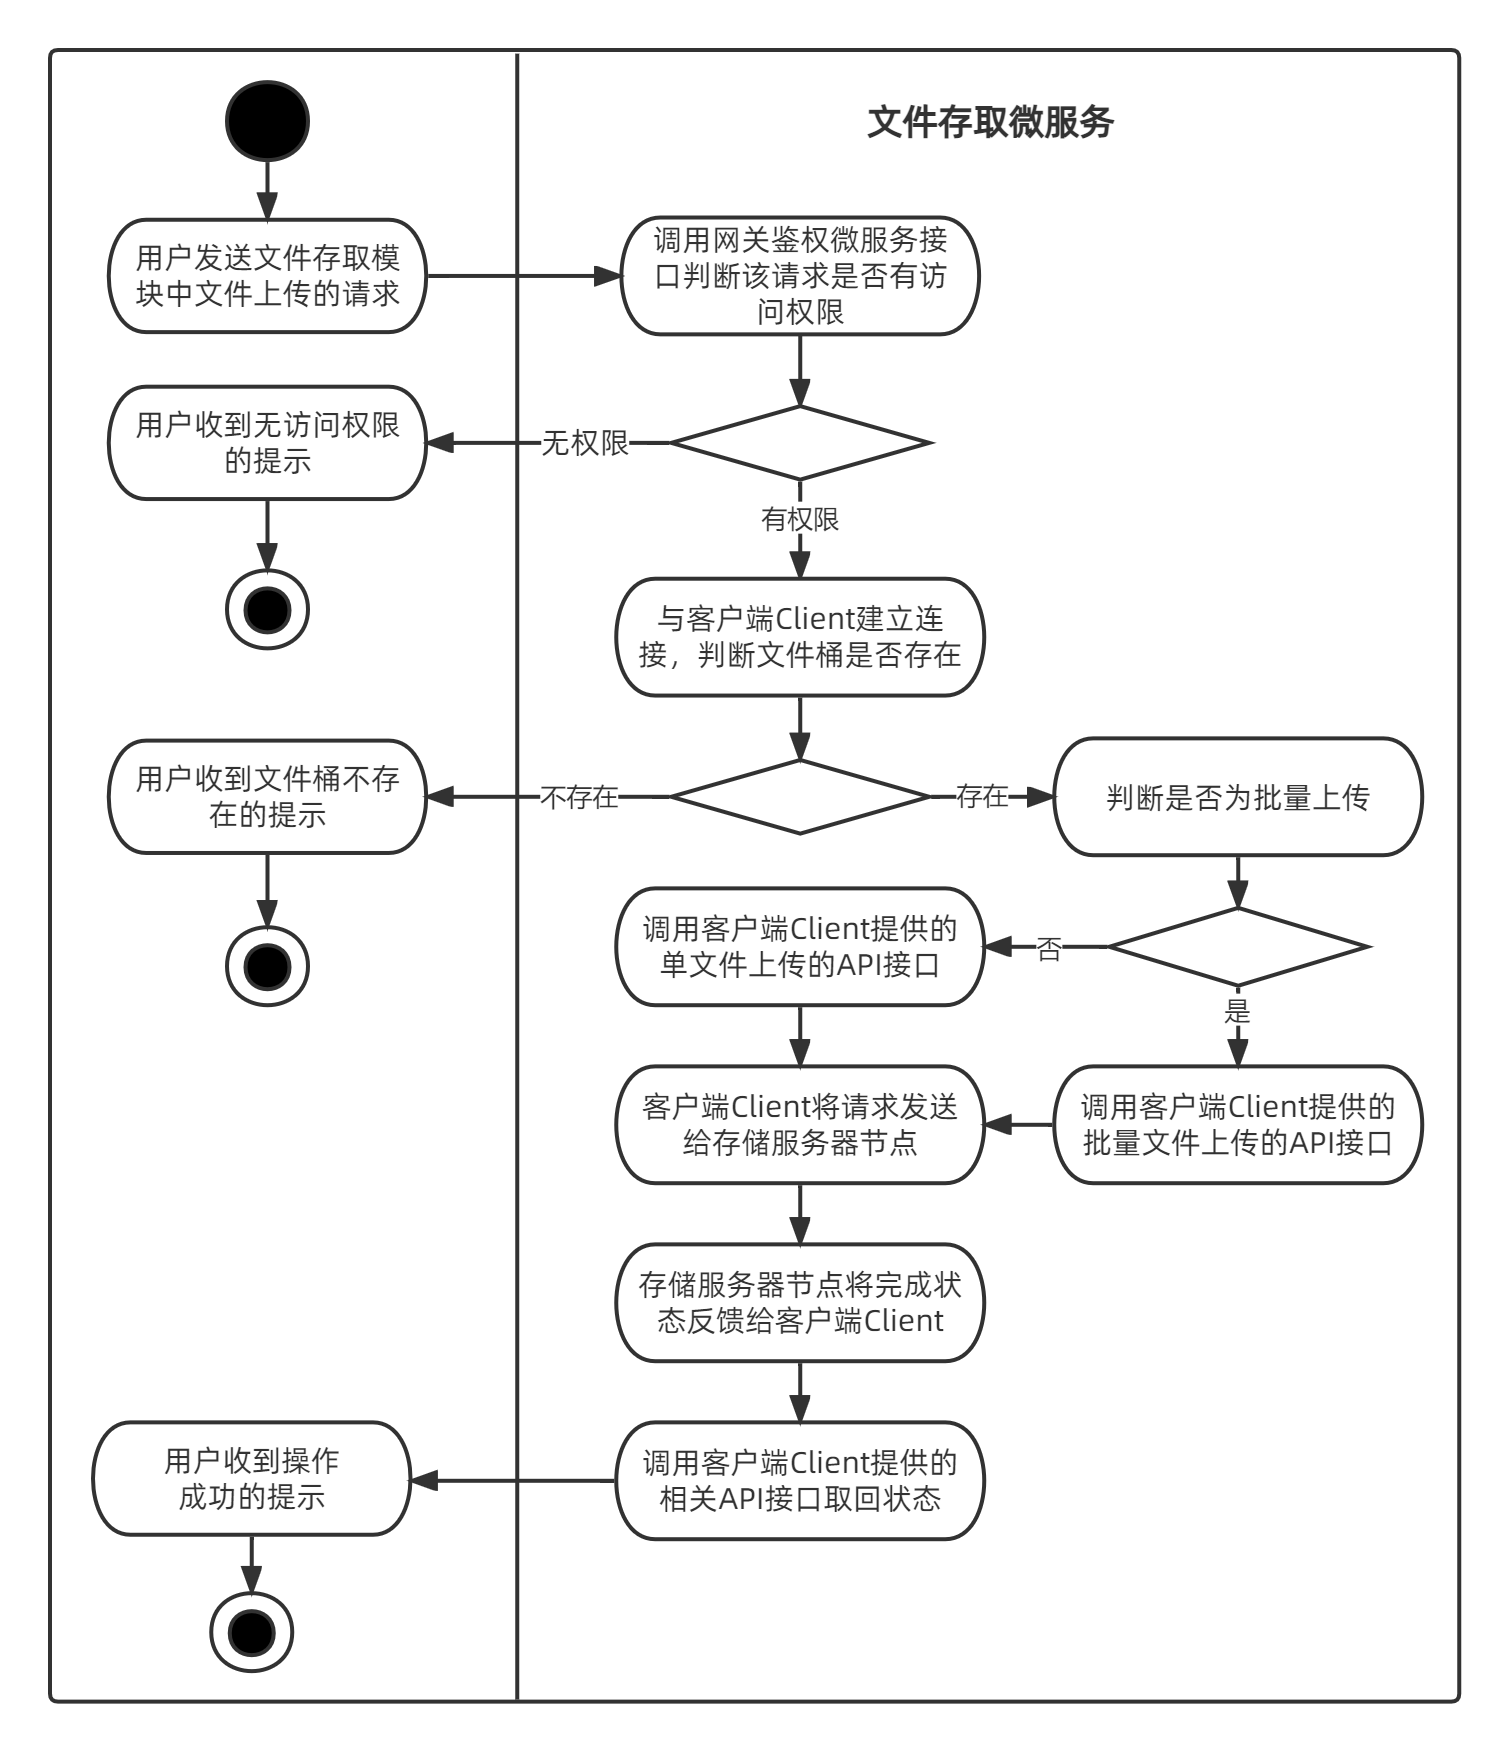
\includegraphics[width=0.7\textwidth]{my_figures/chapter4/文件上传活动图.png}
    \caption{文件上传活动图}
    \label{fig:文件上传活动图}
%     \note{注:图注的内容不宜放到图题中。}
\end{figure}

% 文件上传模块主要负责将用户的文件上传至数据存储服务器中,支持上传多种不同类型的文件,也可以进行多文件批量上传,
文档上传功能是将用户文件上传到对象存储服务器的关键功能之一。在进行文件上传前,需要进行鉴权操作,以确保上传者具备相应的权限。同时,需要对上传的文件进行安全性和完整
性的检查,如文件类型、大小等限制及MD5等校验码的生成和校验。上传成功后,文件需要存储在分布式对象存储系统中,并返回其URL地址以供后续访问使用。
系统能支持用户提交不同形式的文档及实现多文件批量上传。对文件的大小限制也很宽松,一般情况下,只要文件大小不超过1T,即可正常进行上传。在上传过程中,前端能够实时查看
文件上传进度。若遇到网络波动或断线,前端会有相应的反馈通知。在网络出现故障时,系统会暂停文件上传以确保上传结果的正确性。
文件上传活动图如图\ref{fig:文件上传活动图}所示。



(3) 文件下载


文件下载功能主要是把文件从对象存储服务器下载到用户本地。对于文件下载,同样需要进行鉴权操作,确保下载者具备相应的权限。一般用户通过Web界面或者
API接口进行文件下载操作,系统需要根据文件URL地址从分布式对象存储系统中获取对应的文件,并将文件返回给用户。在返回文件时,还需要进行一些安全性和
完整性的检查,如文件大小、MD5等校验码的校验。和文件上传一样,也支持多文件批量下载,在下载过程中前端可以看到文件下载的实时进度,如果遇到网络波动或
断线,前端会有相应的反馈通知,网络故障时,系统会暂停文件的下载。整体的操作流程和文件上传类似。文件下载活动图与文件上传活动图十分类似,此处可参考
文件上传活动图\ref{fig:文件上传活动图}。

% \begin{figure}[htb]
%     \centering
%     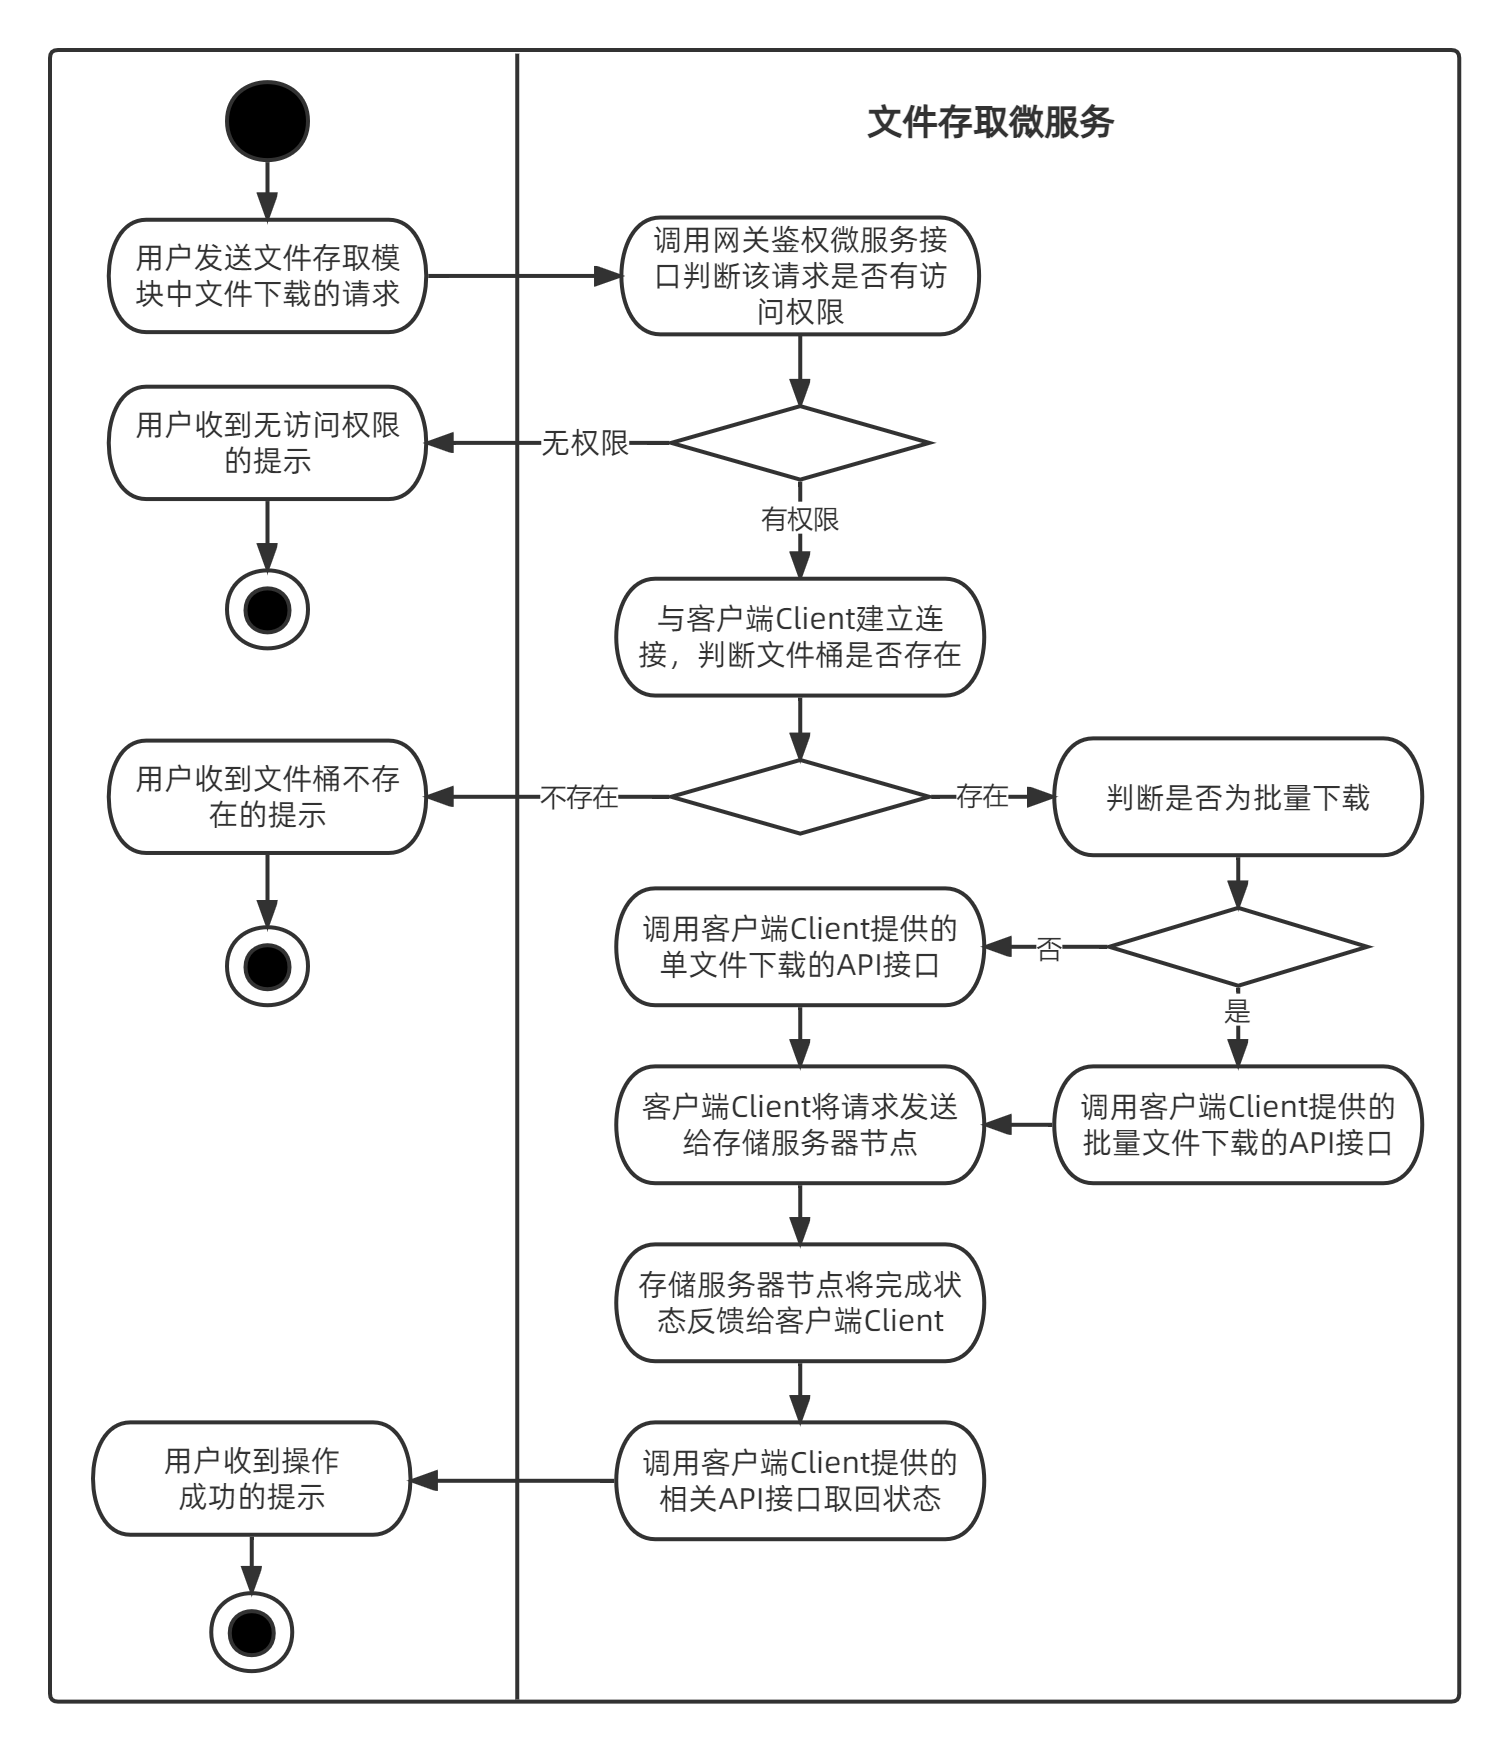
\includegraphics[width=0.7\textwidth]{my_figures/chapter4/文件下载活动图.png}
%     \caption{文件下载活动图}
%     \label{fig:文件下载活动图}
% %     \note{注:图注的内容不宜放到图题中。}
% \end{figure}

% (4) 文件共享

% 文件共享模块主要负责对用户Bucket中的文件进行共享。用户在选中某个文件后,并将其设置为共享,则所有用户均可访问该文件,但文件访问链接是一个
% 临时的共享链接,链接中包含了共享文件的地址、有效期、以及访问密码等信息。用户可以根据自己的需要设置这些参数,然后将链接分享给其他用户。
% 当其他用户或者组织收到共享链接后,需要进行访问授权。授权主要是通过访问密码方式进行。一旦授权通过,用户就可以通过访问
% 共享链接来访问共享文件了。对象存储系统AliIO会根据授权信息来判断用户是否有权访问该文件,如果权限通过,则可以下载或者查看该文件。文件的共享后,其
% 访问策略仍然为文件所属用户设置的策略,任何人无权更改。用户可随时取消文件共享,被用户取消共享或过了有效期的文件将无法访问。对于用户的每一次
% 共享,都会产生一条共享记录,其内容包括共享的文件名、共享的用户、共享的时间等信息。文件共享操作活动图如图\ref{fig:文件共享活动图}所示。

% \begin{figure}[h]
%     \centering
%     \includegraphics[width=0.7\textwidth]{my_figures/chapter4/文件共享活动图.png}
%     \caption{文件共享活动图}
%     \label{fig:文件共享活动图}
% %     \note{注:图注的内容不宜放到图题中。}
% \end{figure}


\subsection{系统监控模块}

\begin{figure}[h]
    \centering
    \includegraphics[width=0.5\textwidth]{my_figures/chapter4/系统监控模块功能结构图.png}
    \caption{系统监控模块功能结构图}
    \label{fig:系统监控模块功能结构图}
%     \note{注:图注的内容不宜放到图题中。}
\end{figure}

系统监控模块主要是对系统运行状态的实时监控、分析和报警,以确保系统运行的稳定性和可靠性。
系统维护模块主要包含三个子模块,分别是状态监控子模块、
记录跟踪子模块和告警通知子模块。只有系统管理员才有该模块的访问权限。系统维护模块的功能结构图如图\ref{fig:系统监控模块功能结构图}所示。


(1)状态监测

% \begin{figure}[h]
%     \centering
%     \includegraphics[width=0.6\textwidth]{my_figures/chapter4/状态监测活动图.png}
%     \caption{状态监测活动图}
%     \label{fig:状态监测活动图}
% %     \note{注:图注的内容不宜放到图题中。}
% \end{figure}


状态监测的主要功能是监测整个存储系统的状态,本系统设置的监控指标有存储桶和对象数量、服务器数量、服务器状态、系统负载、存储容量、吞吐量、响应时间等,
使用监控工具Prometheus进行监控数据
采集和存储,定期对采集的数据进行分析和统计,以便后续数据展示和告警处理。在收集到这些数据后,通过数据可视化工具Grafana将监控数据进行可视化展示,
方便管理员及时了解系统状态,及时发现和解决问题。同时,通过数据分析技术,对数据进行趋势分析、异常检测等,提前发现潜在的问题。



当系统管理员进入系统监测页面时,相应的操作请求首先会通过网关鉴权模块进行权限检查,如果有权限,就会和客户端AliIO-Cli建立连接,调用客户端提供的
查询桶和对象数量、服务器状态、存储容量等相关的API接口,由客户端向对象存储系统AliIO的服务器节点发送命令,通过监控工具Prometheus采集和存储对象
存储服务器相关的状态数据\cite{kongqoji},由数据可视化工具Grafana将监控数据进行可视化展示在页面上\cite{kong2324qoji}。
% 状态监测活动图如图\ref{fig:状态监测活动图}所示。



(2)事件跟踪

事件追踪主要是负责对操作日志、事件日志进行记录和分析,方便系统管理员快速定位和解决问题。在整个管控平台中,日志可以分为两类:系统日志和访问日志。
系统日志记录系统的各种操作和事件,如用户登录、文件上传、权限分配等;访问日志记录用户对文件的访问情况,如文件下载、分享等。针对这两类日志,对象
存储系统管控平台需要提供不同的管理方式。对于系统日志,平台对系统中的各种操作和时间进行收集,并存储到日志数据库中。系统管理员可随时查询日志,并且
系统还提供日志分析功能,会对所有日志进行分析并生成相应的日志报告,让管理员查看系统的运行情况。对于访问日志,平台对用户对文件的访问情况进行收集,
并存储到日志数据库中。系统管理员可根据时间、文件名、用户等条件查询访问日志。同样,系统也会对日志进行分析,并将日志保留一定的时间。



\begin{figure}[htb]
    \centering
    \includegraphics[width=0.6\textwidth]{my_figures/chapter4/记录跟踪活动图.png}
    \caption{事件跟踪活动图}
    \label{fig:记录跟踪活动图}
%     \note{注:图注的内容不宜放到图题中。}
\end{figure}

当系统管理员进入记录跟踪页面时,相应的操作请求首先会通过网关鉴权模块进行权限检查,如果有权限,就会和客户端AliIO-Cli建立连接,调用客户端提供的
日志管理相关的API接口,从日志数据库中取出日志,由对象存储系统AliIO对日志进行分析,并生成相应的日志报告,返回给前端页面。
记录跟踪活动图如图\ref{fig:记录跟踪活动图}所示。



(3)告警通知

告警通知主要负责在系统监测的那些指标出现异常时及时通知管理员或相关负责人,以便快速响应并处理问题,确保系统的稳定性和可靠性。对于系统需要监控的
告警类型,主要就是以状态监测模块中的那些监测指标为主,如磁盘空间不足、系统负载过高、网络连接异常等。系统根据异常类型的紧急程度,定义了不同的告警
级别,如紧急、重要、普通等,以便管理员快速判断和处理问题。当出现告警时,系统会以邮件和短信的形式通知系统管理员\cite{kngqineji}。系统管理员可以在界面上配置告警类
型、级别、通知方式、接收人等信息,还可以去设置触发告警阈值或条件,比如磁盘使用率超过90\%等。系统会记录每一次告警的信息,包括告警类型、级别、时
间、通知方式、接收人、处理结果等,以便后续的跟踪和分析。

当系统监测的指标达到相应的触发条件时,会向系统中设置的接收人发送告警通知,通知的内容包括告警类型标、告警内容、告警级别、发生时间等信息,并将相应的
告警信息存入数据库。告警通知活动图如图\ref{fig:告警通知活动图}所示。

\begin{figure}[htb]
    \centering
    \includegraphics[width=0.6\textwidth]{my_figures/chapter4/告警通知活动图.png}
    \caption{告警通知活动图}
    \label{fig:告警通知活动图}
%     \note{注:图注的内容不宜放到图题中。}
\end{figure}


\section{数据库总体设计}

分布式对象存储系统管控平台需要存储大量的数据信息,这些数据信息包括用户信息、角色信息、权限信息、路由信息、状态信息、日志信息、告警信息等,而且
这些信息也会随着用户的增多而逐渐增加,这些数据无论是对用户还是对系统管理人员都是尤为重要的。因此,良好的数据库设计可以有效的管理这些重要的数据
信息,提高系统的效率和稳定性。结合本系统的需求特点,最终选用MySQL数据库进行后台数据的管理。MySQL是一种关系型数据库管理系统(RDBMS),它是一个
开源的、基于客户端-服务器模型的数据库系统\cite{kn2e2i},大可以处理大量数据和并发用户,同时具有自动故障转移和备份恢复功能,可确保数据的可靠性和完整性。
由于MySQL具有高性能、可靠性、安全性、可扩展性等优点,成为本系统首选的数据库管理系统。

% \subsection{数据库E-R图设计}

在数据库设计过程中,实体-关系图(E-R图)的绘制是不可省略的步骤,它用于描述实体(Entity)和实体之间的关系(Relationship)\cite{kng2eji},该建模工具让开发者
更清晰的理解和梳理数据之间的关系。根据需求分析可知,本系统的实体有用户、角色、权限、策略、存储桶、存储服务器、日志信息、告警信息,各实体之间的
关系(即E-R图)如图\ref{fig:E-R图}所示。

\begin{figure}[htb]
    \centering
    \includegraphics[width=1\textwidth]{my_figures/chapter4/E-R图.png}
    \caption{分布式对象存储系统管控平台E-R图}
    \label{fig:E-R图}
%     \note{注:图注的内容不宜放到图题中。}
\end{figure}

\section{本章小结}

本章重点介绍分布式对象存储系统管控平台的系统架构与设计,为后续的开发工作提供概要设计和基础依据。首先,通过分析系统架构图,详细介绍了系统的逻辑架构和后端的技术架构,
并对各个模块的功能模块设计进行了梳理。然后,基于各个功能模块的功能结构图和UML活动图,进一步深入介绍了各个功能模块的具体设计,包括注册认证模块、权限控制模块、策略
控制模块、文件存取模块以及系统监控模块。最后,通过E-R图形式对数据库表之间的关系进行了说明。本章对分布式对象存储系统管控平台进行了概要设计,为后面的详细设计提供了
依据。